%*************************************************************************
% A Classic Thesis Style
% An Homage to The Elements of Typographic Style
%
% Copyright (C) 2017 André Miede and Ivo Pletikosić
%
% If you like the style then I would appreciate a postcard. My address
% can be found in the file ClassicThesis.pdf. A collection of the
% postcards I received so far is available online at
% http://postcards.miede.de
%
% License:F
% This program is free software; you can redistribute it and/or modify
% it under the terms of the GNU General Public License as published by
% the Free Software Foundation; either version 2 of the License, or
% (at your option) any later version.
%
% This program is distributed in the hope that it will be useful,
% but WITHOUT ANY WARRANTY; without even the implied warranty of
% MERCHANTABILITY or FITNESS FOR A PARTICULAR PURPOSE.  See the
% GNU General Public License for more details.
%
% You should have received a copy of the GNU General Public License
% along with this program; see the file COPYING.  If not, write to
% the Free Software Foundation, Inc., 59 Temple Place - Suite 330,
% Boston, MA 02111-1307, USA.
%
% PLEASE SEE ALSO THE AUTHORS' NOTE REGARDING THIS LICENSE
% IN THE DOCUMENTATION (ClassicThesis.pdf --> Chapter 1 / Chapter01.tex)
%*************************************************************************
\RequirePackage{silence} % :-\
    \WarningFilter{scrreprt}{Usage of package `titlesec'}
    %\WarningFilter{scrreprt}{Activating an ugly workaround}
    \WarningFilter{titlesec}{Non standard sectioning command detected}
\documentclass[ openright,titlepage,numbers=noenddot,headinclude,%twoside, %1headlines,% letterpaper a4paper
                footinclude=true,cleardoublepage=empty,
                BCOR=5mm,paper=a4,fontsize=11pt,%11pt,a4paper,%
                ngerman,american,%lockflag%
                ]{scrreprt}

%*************************************************************************
% Note: Make all your adjustments in here
%*************************************************************************
% ****************************************************************************************************
% hdathesis-config.tex 
% Use it at the beginning of your thesis.tex, or as a LaTeX Preamble 
% in your thesis.{tex,lyx} with % ****************************************************************************************************
% hdathesis-config.tex 
% Use it at the beginning of your thesis.tex, or as a LaTeX Preamble 
% in your thesis.{tex,lyx} with % ****************************************************************************************************
% hdathesis-config.tex 
% Use it at the beginning of your thesis.tex, or as a LaTeX Preamble 
% in your thesis.{tex,lyx} with \input{hdathesis-config}
% ****************************************************************************************************

% ****************************************************************************************************
% 1. Personal data and user ad-hoc commands
% ****************************************************************************************************
\newcommand{\myTitle}{A Modular Classification Pipeline with Embedded Continuous Learning\xspace}
%\newcommand{\mySubtitle}{An Homage to The Elements of Typographic Style\xspace}
\newcommand{\myDegree}{Bachelor of Science (B.\,Sc.)\xspace} 
%\newcommand{\myDegree}{Bachelor of Arts (B.\,A.)\xspace}
%\newcommand{\myDegree}{Master of Science (M.\,Sc.)\xspace}
%\newcommand{\myDegree}{Master of Arts (M.\,A.)\xspace}
\newcommand{\myName}{Dajlan Zaimaj\xspace}
\newcommand{\myId}{1121743\xspace}
\newcommand{\myProf}{Prof. Dr. Yvonne Jung\xspace}
\newcommand{\myOtherProf}{Prof. Dr. Ralf Kundel\xspace}
\newcommand{\myFaculty}{Fachbereich Informatik\xspace}
\newcommand{\myUni}{Hochschule Darmstadt\xspace}
\newcommand{\myLocation}{Darmstadt\xspace}
\newcommand{\myTime}{\today\xspace}
\newcommand{\myVersion}{version 1.0\xspace}

% ****************************************************************************************************
% 2. Is it a master thesis?
% ****************************************************************************************************
%\PassOptionsToPackage{master}{hdathesis} % uncomment if this is a master thesis 

% ****************************************************************************************************
% 3. Does the thesis have a lock flag?
% ****************************************************************************************************
%\PassOptionsToPackage{lockflag}{hdathesis} % uncomment if this thesis has a lock flag 

% ****************************************************************************************************
% 4. Loading some handy packages
% ****************************************************************************************************
% ****************************************************************************************************
% Packages with options that might require adjustments
% ****************************************************************************************************

%\PassOptionsToPackage{ngerman,american}{babel}   % change this to your language(s)
% Spanish languages need extra options in order to work with this template
%\PassOptionsToPackage{spanish,es-lcroman}{babel}
\usepackage{babel}


% ****************************************************************************************************

% ****************************************************************************************************
% 1. Personal data and user ad-hoc commands
% ****************************************************************************************************
\newcommand{\myTitle}{A Modular Classification Pipeline with Embedded Continuous Learning\xspace}
%\newcommand{\mySubtitle}{An Homage to The Elements of Typographic Style\xspace}
\newcommand{\myDegree}{Bachelor of Science (B.\,Sc.)\xspace} 
%\newcommand{\myDegree}{Bachelor of Arts (B.\,A.)\xspace}
%\newcommand{\myDegree}{Master of Science (M.\,Sc.)\xspace}
%\newcommand{\myDegree}{Master of Arts (M.\,A.)\xspace}
\newcommand{\myName}{Dajlan Zaimaj\xspace}
\newcommand{\myId}{1121743\xspace}
\newcommand{\myProf}{Prof. Dr. Yvonne Jung\xspace}
\newcommand{\myOtherProf}{Prof. Dr. Ralf Kundel\xspace}
\newcommand{\myFaculty}{Fachbereich Informatik\xspace}
\newcommand{\myUni}{Hochschule Darmstadt\xspace}
\newcommand{\myLocation}{Darmstadt\xspace}
\newcommand{\myTime}{\today\xspace}
\newcommand{\myVersion}{version 1.0\xspace}

% ****************************************************************************************************
% 2. Is it a master thesis?
% ****************************************************************************************************
%\PassOptionsToPackage{master}{hdathesis} % uncomment if this is a master thesis 

% ****************************************************************************************************
% 3. Does the thesis have a lock flag?
% ****************************************************************************************************
%\PassOptionsToPackage{lockflag}{hdathesis} % uncomment if this thesis has a lock flag 

% ****************************************************************************************************
% 4. Loading some handy packages
% ****************************************************************************************************
% ****************************************************************************************************
% Packages with options that might require adjustments
% ****************************************************************************************************

%\PassOptionsToPackage{ngerman,american}{babel}   % change this to your language(s)
% Spanish languages need extra options in order to work with this template
%\PassOptionsToPackage{spanish,es-lcroman}{babel}
\usepackage{babel}


% ****************************************************************************************************

% ****************************************************************************************************
% 1. Personal data and user ad-hoc commands
% ****************************************************************************************************
\newcommand{\myTitle}{A Modular Classification Pipeline with Embedded Continuous Learning\xspace}
%\newcommand{\mySubtitle}{An Homage to The Elements of Typographic Style\xspace}
\newcommand{\myDegree}{Bachelor of Science (B.\,Sc.)\xspace} 
%\newcommand{\myDegree}{Bachelor of Arts (B.\,A.)\xspace}
%\newcommand{\myDegree}{Master of Science (M.\,Sc.)\xspace}
%\newcommand{\myDegree}{Master of Arts (M.\,A.)\xspace}
\newcommand{\myName}{Dajlan Zaimaj\xspace}
\newcommand{\myId}{1121743\xspace}
\newcommand{\myProf}{Prof. Dr. Yvonne Jung\xspace}
\newcommand{\myOtherProf}{Prof. Dr. Ralf Kundel\xspace}
\newcommand{\myFaculty}{Fachbereich Informatik\xspace}
\newcommand{\myUni}{Hochschule Darmstadt\xspace}
\newcommand{\myLocation}{Darmstadt\xspace}
\newcommand{\myTime}{\today\xspace}
\newcommand{\myVersion}{version 1.0\xspace}

% ****************************************************************************************************
% 2. Is it a master thesis?
% ****************************************************************************************************
%\PassOptionsToPackage{master}{hdathesis} % uncomment if this is a master thesis 

% ****************************************************************************************************
% 3. Does the thesis have a lock flag?
% ****************************************************************************************************
%\PassOptionsToPackage{lockflag}{hdathesis} % uncomment if this thesis has a lock flag 

% ****************************************************************************************************
% 4. Loading some handy packages
% ****************************************************************************************************
% ****************************************************************************************************
% Packages with options that might require adjustments
% ****************************************************************************************************

%\PassOptionsToPackage{ngerman,american}{babel}   % change this to your language(s)
% Spanish languages need extra options in order to work with this template
%\PassOptionsToPackage{spanish,es-lcroman}{babel}
\usepackage{babel}


% ****************************************************************************************************
% classicthesis-config.tex
% formerly known as loadpackages.sty, classicthesis-ldpkg.sty, and classicthesis-preamble.sty
% Use it at the beginning of your ClassicThesis.tex, or as a LaTeX Preamble
% in your ClassicThesis.{tex,lyx} with % ****************************************************************************************************
% classicthesis-config.tex
% formerly known as loadpackages.sty, classicthesis-ldpkg.sty, and classicthesis-preamble.sty
% Use it at the beginning of your ClassicThesis.tex, or as a LaTeX Preamble
% in your ClassicThesis.{tex,lyx} with % ****************************************************************************************************
% classicthesis-config.tex
% formerly known as loadpackages.sty, classicthesis-ldpkg.sty, and classicthesis-preamble.sty
% Use it at the beginning of your ClassicThesis.tex, or as a LaTeX Preamble
% in your ClassicThesis.{tex,lyx} with \input{classicthesis-config}
% ****************************************************************************************************
% If you like the classicthesis, then I would appreciate a postcard.
% My address can be found in the file ClassicThesis.pdf. A collection
% of the postcards I received so far is available online at
% http://postcards.miede.de
% ****************************************************************************************************


% ****************************************************************************************************
% 0. Set the encoding of your files. UTF-8 is the only sensible encoding nowadays. If you can't read
% äöüßáéçèê∂åëæƒÏ€ then change the encoding setting in your editor, not the line below. If your editor
% does not support utf8 use another editor!
% ****************************************************************************************************
\PassOptionsToPackage{utf8}{inputenc}
\usepackage{inputenc}

% ****************************************************************************************************
% 1. Configure classicthesis for your needs here, e.g., remove "drafting" below
% in order to deactivate the time-stamp on the pages
% (see ClassicThesis.pdf for more information):
% ****************************************************************************************************
\PassOptionsToPackage{
    drafting=false,   % print version information on the bottom of the pages
    tocaligned=false, % the left column of the toc will be aligned (no indentation)
    dottedtoc=true,   % page numbers in ToC flushed right
    parts=true,       % use part division
    eulerchapternumbers=true, % use AMS Euler for chapter font (otherwise Palatino)
    linedheaders=false,       % chaper headers will have line above and beneath
    floatperchapter=true,     % numbering per chapter for all floats (i.e., Figure 1.1)
    listings=false,    % load listings package and setup LoL
    subfig=true,      % setup for preloaded subfig package
    eulermath=false,  % use awesome Euler fonts for mathematical formulae (only with pdfLaTeX)
    beramono=true,    % toggle a nice monospaced font (w/ bold)
    minionpro=false   % setup for minion pro font; use minion pro small caps as well (only with pdfLaTeX)
}{classicthesis}


% ****************************************************************************************************
% 2. Personal data and user ad-hoc commands
% ****************************************************************************************************
%\newcommand{\myTitle}{A Classic Thesis Style\xspace}
%\newcommand{\mySubtitle}{An Homage to The Elements of Typographic Style\xspace}
%\newcommand{\myDegree}{Doktor-Ingenieur (Dr.-Ing.)\xspace}
%\newcommand{\myName}{André Miede\xspace}
%\newcommand{\myProf}{Put name here\xspace}
%\newcommand{\myOtherProf}{Put name here\xspace}
%\newcommand{\mySupervisor}{Put name here\xspace}
%\newcommand{\myFaculty}{Put data here\xspace}
%\newcommand{\myDepartment}{Put data here\xspace}
%\newcommand{\myUni}{Put data here\xspace}
%\newcommand{\myLocation}{Saarbrücken\xspace}
%\newcommand{\myTime}{October 2017\xspace}
%\newcommand{\myVersion}{version 4.4}

% ********************************************************************
% Setup, finetuning, and useful commands
% ********************************************************************
\newcounter{dummy} % necessary for correct hyperlinks (to index, bib, etc.)
\newlength{\abcd} % for ab..z string length calculation
\providecommand{\mLyX}{L\kern-.1667em\lower.25em\hbox{Y}\kern-.125emX\@}
\newcommand{\ie}{i.\,e.}
\newcommand{\Ie}{I.\,e.}
\newcommand{\eg}{e.\,g.}
\newcommand{\Eg}{E.\,g.}
% ****************************************************************************************************


% ****************************************************************************************************
% 3. Loading some handy packages
% ****************************************************************************************************
% ********************************************************************
% Packages with options that might require adjustments
% ********************************************************************
%\PassOptionsToPackage{ngerman,american}{babel}   % change this to your language(s), main language last
% Spanish languages need extra options in order to work with this template
%\PassOptionsToPackage{spanish,es-lcroman}{babel}
\usepackage{babel}

\usepackage{csquotes}
\usepackage{placeins}


\PassOptionsToPackage{%
    %backend=biber,bibencoding=utf8, %instead of bibtex
    backend=bibtex8,bibencoding=ascii,%
    language=auto,%
    %style=numeric-comp,%
    style=alphabetic,%
    %style=authoryear-comp, % Author 1999, 2010
    %bibstyle=authoryear,dashed=false, % dashed: substitute rep. author with ---
    sorting=nyt, % name, year, title
    maxbibnames=10, % default: 3, et al.
    %backref=true,%
    natbib=true % natbib compatibility mode (\citep and \citet still work)
}{biblatex}
\usepackage{biblatex}

\PassOptionsToPackage{fleqn}{amsmath}       % math environments and more by the AMS
\usepackage{amsmath}

\PassOptionsToPackage{doublespacing}{hdathesis}  % options: abbrev exam big wiwi english master
\usepackage{hdathesis}

% ********************************************************************
% General useful packages
% ********************************************************************
\PassOptionsToPackage{T1}{fontenc} % T2A for cyrillics
\usepackage{fontenc}
\usepackage{textcomp} % fix warning with missing font shapes
\usepackage{scrhack} % fix warnings when using KOMA with listings package
\usepackage{xspace} % to get the spacing after macros right
\usepackage{mparhack} % get marginpar right
%\usepackage{fixltx2e} % fixes some LaTeX stuff --> since 2015 in the LaTeX kernel (see below)
% \usepackage[latest]{latexrelease} % emulate newer kernel version if older is detected
\PassOptionsToPackage{smaller}{acronym}
\usepackage{acronym} % nice macros for handling all acronyms in the thesis
%\renewcommand{\bflabel}[1]{{#1}\hfill} % fix the list of acronyms --> no longer working
%\renewcommand*{\acsfont}[1]{\textsc{#1}}
%\renewcommand*{\aclabelfont}[1]{\acsfont{#1}}
%\def\bflabel#1{{#1\hfill}}
\def\bflabel#1{{\acsfont{#1}\hfill}}
\def\aclabelfont#1{\acsfont{#1}}
% ****************************************************************************************************
%\usepackage{pgfplots} % External TikZ/PGF support (thanks to Andreas Nautsch)
%\usetikzlibrary{external}
%\tikzexternalize[mode=list and make, prefix=ext-tikz/]
% ****************************************************************************************************

\usepackage{longtable,booktabs}
% ****************************************************************************************************
% 4. Setup floats: tables, (sub)figures, and captions
% ****************************************************************************************************
\usepackage{tabularx} % better tables
\setlength{\extrarowheight}{3pt} % increase table row height
\newcommand{\tableheadline}[1]{\multicolumn{1}{c}{\spacedlowsmallcaps{#1}}}
\newcommand{\myfloatalign}{\centering} % to be used with each float for alignment
\usepackage{caption}
% Thanks to cgnieder and Claus Lahiri
% http://tex.stackexchange.com/questions/69349/spacedlowsmallcaps-in-caption-label
% [REMOVED DUE TO OTHER PROBLEMS, SEE ISSUE #82]
%\DeclareCaptionLabelFormat{smallcaps}{\bothIfFirst{#1}{~}\MakeTextLowercase{\textsc{#2}}}
%\captionsetup{font=small,labelformat=smallcaps} % format=hang,
\captionsetup{font=small} % format=hang,
\usepackage{subfig}
% ****************************************************************************************************


% ****************************************************************************************************
% 5. Setup code listings
% ****************************************************************************************************
\usepackage{listings}
%\lstset{emph={trueIndex,root},emphstyle=\color{BlueViolet}}%\underbar} % for special keywords
\lstset{language=[LaTeX]Tex,%C++,
    morekeywords={PassOptionsToPackage,selectlanguage},
    keywordstyle=\color{RoyalBlue},%\bfseries,
    basicstyle=\small\ttfamily,
    %identifierstyle=\color{NavyBlue},
    commentstyle=\color{Green}\ttfamily,
    stringstyle=\rmfamily,
    numbers=none,%left,%
    numberstyle=\scriptsize,%\tiny
    stepnumber=5,
    numbersep=8pt,
    showstringspaces=false,
    breaklines=true,
    %frameround=ftff,
    %frame=single,
    belowcaptionskip=.75\baselineskip
    %frame=L
}
% ****************************************************************************************************


% ****************************************************************************************************
% 6. PDFLaTeX, hyperreferences, and citation backreferences
% ****************************************************************************************************
% ********************************************************************
% Using PDFLaTeX
% ********************************************************************
\PassOptionsToPackage{hyperfootnotes=false,pdfpagelabels}{hyperref}
\usepackage{hyperref}  % backref linktocpage pagebackref
%\ifpdf
%\pdfcompresslevel=9
%\pdfadjustspacing=1
%\fi
%\PassOptionsToPackage{pdftex}{graphicx} %%%IVO: driver will be chosen automatically
\usepackage{graphicx}


% ********************************************************************
% Hyperreferences
% ********************************************************************
\hypersetup{%
    %draft, % hyperref's draft mode, for printing see below
    colorlinks=true, linktocpage=true, pdfstartpage=3, pdfstartview=FitV,%
    % uncomment the following line if you want to have black links (e.g., for printing)
    %colorlinks=false, linktocpage=false, pdfstartpage=3, pdfstartview=FitV, pdfborder={0 0 0},%
    breaklinks=true, pdfpagemode=UseNone, pageanchor=true, pdfpagemode=UseOutlines,%
    plainpages=false, bookmarksnumbered, bookmarksopen=true, bookmarksopenlevel=1,%
    hypertexnames=true, pdfhighlight=/O,%nesting=true,%frenchlinks,%
    urlcolor=webbrown, linkcolor=RoyalBlue, citecolor=webgreen, %pagecolor=RoyalBlue,%
    %urlcolor=Black, linkcolor=Black, citecolor=Black, %pagecolor=Black,%
    pdftitle={\myTitle},%
    pdfauthor={\textcopyright\ \myName, \myUni, \myFaculty},%
    pdfsubject={},%
    pdfkeywords={},%
    pdfcreator={pdfLaTeX},%
    pdfproducer={LaTeX with hyperref and classicthesis}%
}

% ********************************************************************
% Setup autoreferences
% ********************************************************************
% There are some issues regarding autorefnames
% http://www.ureader.de/msg/136221647.aspx
% http://www.tex.ac.uk/cgi-bin/texfaq2html?label=latexwords
% you have to redefine the makros for the
% language you use, e.g., american, ngerman
% (as chosen when loading babel/AtBeginDocument)
% ********************************************************************
\makeatletter
\@ifpackageloaded{babel}%
{%
    \addto\extrasamerican{%
        \renewcommand*{\figureautorefname}{Figure}%
        \renewcommand*{\tableautorefname}{Table}%
        \renewcommand*{\partautorefname}{Part}%
        \renewcommand*{\chapterautorefname}{Chapter}%
        \renewcommand*{\sectionautorefname}{Section}%
        \renewcommand*{\subsectionautorefname}{Section}%
        \renewcommand*{\subsubsectionautorefname}{Section}%
    }%
    \addto\extrasngerman{%
        \renewcommand*{\paragraphautorefname}{Figure}%
        \renewcommand*{\subparagraphautorefname}{Table}%
        \renewcommand*{\footnoteautorefname}{Footnote}%
        \renewcommand*{\FancyVerbLineautorefname}{Rows}%
        \renewcommand*{\theoremautorefname}{Theorem}%
        \renewcommand*{\appendixautorefname}{Appendix}%
        \renewcommand*{\equationautorefname}{Equation}%
        \renewcommand*{\itemautorefname}{Punkt}%
    }%
    % Fix to getting autorefs for subfigures right (thanks to Belinda Vogt for changing the definition)
    \providecommand{\subfigureautorefname}{\figureautorefname}%
}{\relax}
\makeatother


% ****************************************************************************************************
% 7. Last calls before the bar closes
% ****************************************************************************************************
% ********************************************************************
% Development Stuff
% ********************************************************************
\listfiles
%\PassOptionsToPackage{l2tabu,orthodox,abort}{nag}
%  \usepackage{nag}
%\PassOptionsToPackage{warning, all}{onlyamsmath}
%  \usepackage{onlyamsmath}

% ********************************************************************
% Last, but not least...
% ********************************************************************
\usepackage{classicthesis}
% ****************************************************************************************************


% ****************************************************************************************************
% 8. Further adjustments (experimental)
% ****************************************************************************************************
% ********************************************************************
% Changing the text area
% ********************************************************************
%\areaset[current]{312pt}{761pt} % 686 (factor 2.2) + 33 head + 42 head \the\footskip
%\setlength{\marginparwidth}{7em}%
%\setlength{\marginparsep}{2em}%

% ********************************************************************
% Using different fonts
% ********************************************************************
%\usepackage[oldstylenums]{kpfonts} % oldstyle notextcomp
%\usepackage[osf]{libertine}
%\usepackage[light,condensed,math]{iwona}
%\renewcommand{\sfdefault}{iwona}
%\usepackage{lmodern} % <-- no osf support :-(
%\usepackage{cfr-lm} %
%\usepackage[urw-garamond]{mathdesign} <-- no osf support :-(
%\usepackage[default,osfigures]{opensans} % scale=0.95
%\usepackage[sfdefault]{FiraSans}
% ********************************************************************
% \usepackage[largesc,osf]{newpxtext}
% Used to fix these:
% https://bitbucket.org/amiede/classicthesis/issues/139/italics-in-pallatino-capitals-chapter
% https://bitbucket.org/amiede/classicthesis/issues/45/problema-testatine-su-classicthesis-style
% ********************************************************************
%\linespread{1.05} % a bit more for Palatino
% ****************************************************************************************************

% ****************************************************************************************************
% If you like the classicthesis, then I would appreciate a postcard.
% My address can be found in the file ClassicThesis.pdf. A collection
% of the postcards I received so far is available online at
% http://postcards.miede.de
% ****************************************************************************************************


% ****************************************************************************************************
% 0. Set the encoding of your files. UTF-8 is the only sensible encoding nowadays. If you can't read
% äöüßáéçèê∂åëæƒÏ€ then change the encoding setting in your editor, not the line below. If your editor
% does not support utf8 use another editor!
% ****************************************************************************************************
\PassOptionsToPackage{utf8}{inputenc}
\usepackage{inputenc}

% ****************************************************************************************************
% 1. Configure classicthesis for your needs here, e.g., remove "drafting" below
% in order to deactivate the time-stamp on the pages
% (see ClassicThesis.pdf for more information):
% ****************************************************************************************************
\PassOptionsToPackage{
    drafting=false,   % print version information on the bottom of the pages
    tocaligned=false, % the left column of the toc will be aligned (no indentation)
    dottedtoc=true,   % page numbers in ToC flushed right
    parts=true,       % use part division
    eulerchapternumbers=true, % use AMS Euler for chapter font (otherwise Palatino)
    linedheaders=false,       % chaper headers will have line above and beneath
    floatperchapter=true,     % numbering per chapter for all floats (i.e., Figure 1.1)
    listings=false,    % load listings package and setup LoL
    subfig=true,      % setup for preloaded subfig package
    eulermath=false,  % use awesome Euler fonts for mathematical formulae (only with pdfLaTeX)
    beramono=true,    % toggle a nice monospaced font (w/ bold)
    minionpro=false   % setup for minion pro font; use minion pro small caps as well (only with pdfLaTeX)
}{classicthesis}


% ****************************************************************************************************
% 2. Personal data and user ad-hoc commands
% ****************************************************************************************************
%\newcommand{\myTitle}{A Classic Thesis Style\xspace}
%\newcommand{\mySubtitle}{An Homage to The Elements of Typographic Style\xspace}
%\newcommand{\myDegree}{Doktor-Ingenieur (Dr.-Ing.)\xspace}
%\newcommand{\myName}{André Miede\xspace}
%\newcommand{\myProf}{Put name here\xspace}
%\newcommand{\myOtherProf}{Put name here\xspace}
%\newcommand{\mySupervisor}{Put name here\xspace}
%\newcommand{\myFaculty}{Put data here\xspace}
%\newcommand{\myDepartment}{Put data here\xspace}
%\newcommand{\myUni}{Put data here\xspace}
%\newcommand{\myLocation}{Saarbrücken\xspace}
%\newcommand{\myTime}{October 2017\xspace}
%\newcommand{\myVersion}{version 4.4}

% ********************************************************************
% Setup, finetuning, and useful commands
% ********************************************************************
\newcounter{dummy} % necessary for correct hyperlinks (to index, bib, etc.)
\newlength{\abcd} % for ab..z string length calculation
\providecommand{\mLyX}{L\kern-.1667em\lower.25em\hbox{Y}\kern-.125emX\@}
\newcommand{\ie}{i.\,e.}
\newcommand{\Ie}{I.\,e.}
\newcommand{\eg}{e.\,g.}
\newcommand{\Eg}{E.\,g.}
% ****************************************************************************************************


% ****************************************************************************************************
% 3. Loading some handy packages
% ****************************************************************************************************
% ********************************************************************
% Packages with options that might require adjustments
% ********************************************************************
%\PassOptionsToPackage{ngerman,american}{babel}   % change this to your language(s), main language last
% Spanish languages need extra options in order to work with this template
%\PassOptionsToPackage{spanish,es-lcroman}{babel}
\usepackage{babel}

\usepackage{csquotes}
\usepackage{placeins}


\PassOptionsToPackage{%
    %backend=biber,bibencoding=utf8, %instead of bibtex
    backend=bibtex8,bibencoding=ascii,%
    language=auto,%
    %style=numeric-comp,%
    style=alphabetic,%
    %style=authoryear-comp, % Author 1999, 2010
    %bibstyle=authoryear,dashed=false, % dashed: substitute rep. author with ---
    sorting=nyt, % name, year, title
    maxbibnames=10, % default: 3, et al.
    %backref=true,%
    natbib=true % natbib compatibility mode (\citep and \citet still work)
}{biblatex}
\usepackage{biblatex}

\PassOptionsToPackage{fleqn}{amsmath}       % math environments and more by the AMS
\usepackage{amsmath}

\PassOptionsToPackage{doublespacing}{hdathesis}  % options: abbrev exam big wiwi english master
\usepackage{hdathesis}

% ********************************************************************
% General useful packages
% ********************************************************************
\PassOptionsToPackage{T1}{fontenc} % T2A for cyrillics
\usepackage{fontenc}
\usepackage{textcomp} % fix warning with missing font shapes
\usepackage{scrhack} % fix warnings when using KOMA with listings package
\usepackage{xspace} % to get the spacing after macros right
\usepackage{mparhack} % get marginpar right
%\usepackage{fixltx2e} % fixes some LaTeX stuff --> since 2015 in the LaTeX kernel (see below)
% \usepackage[latest]{latexrelease} % emulate newer kernel version if older is detected
\PassOptionsToPackage{smaller}{acronym}
\usepackage{acronym} % nice macros for handling all acronyms in the thesis
%\renewcommand{\bflabel}[1]{{#1}\hfill} % fix the list of acronyms --> no longer working
%\renewcommand*{\acsfont}[1]{\textsc{#1}}
%\renewcommand*{\aclabelfont}[1]{\acsfont{#1}}
%\def\bflabel#1{{#1\hfill}}
\def\bflabel#1{{\acsfont{#1}\hfill}}
\def\aclabelfont#1{\acsfont{#1}}
% ****************************************************************************************************
%\usepackage{pgfplots} % External TikZ/PGF support (thanks to Andreas Nautsch)
%\usetikzlibrary{external}
%\tikzexternalize[mode=list and make, prefix=ext-tikz/]
% ****************************************************************************************************

\usepackage{longtable,booktabs}
% ****************************************************************************************************
% 4. Setup floats: tables, (sub)figures, and captions
% ****************************************************************************************************
\usepackage{tabularx} % better tables
\setlength{\extrarowheight}{3pt} % increase table row height
\newcommand{\tableheadline}[1]{\multicolumn{1}{c}{\spacedlowsmallcaps{#1}}}
\newcommand{\myfloatalign}{\centering} % to be used with each float for alignment
\usepackage{caption}
% Thanks to cgnieder and Claus Lahiri
% http://tex.stackexchange.com/questions/69349/spacedlowsmallcaps-in-caption-label
% [REMOVED DUE TO OTHER PROBLEMS, SEE ISSUE #82]
%\DeclareCaptionLabelFormat{smallcaps}{\bothIfFirst{#1}{~}\MakeTextLowercase{\textsc{#2}}}
%\captionsetup{font=small,labelformat=smallcaps} % format=hang,
\captionsetup{font=small} % format=hang,
\usepackage{subfig}
% ****************************************************************************************************


% ****************************************************************************************************
% 5. Setup code listings
% ****************************************************************************************************
\usepackage{listings}
%\lstset{emph={trueIndex,root},emphstyle=\color{BlueViolet}}%\underbar} % for special keywords
\lstset{language=[LaTeX]Tex,%C++,
    morekeywords={PassOptionsToPackage,selectlanguage},
    keywordstyle=\color{RoyalBlue},%\bfseries,
    basicstyle=\small\ttfamily,
    %identifierstyle=\color{NavyBlue},
    commentstyle=\color{Green}\ttfamily,
    stringstyle=\rmfamily,
    numbers=none,%left,%
    numberstyle=\scriptsize,%\tiny
    stepnumber=5,
    numbersep=8pt,
    showstringspaces=false,
    breaklines=true,
    %frameround=ftff,
    %frame=single,
    belowcaptionskip=.75\baselineskip
    %frame=L
}
% ****************************************************************************************************


% ****************************************************************************************************
% 6. PDFLaTeX, hyperreferences, and citation backreferences
% ****************************************************************************************************
% ********************************************************************
% Using PDFLaTeX
% ********************************************************************
\PassOptionsToPackage{hyperfootnotes=false,pdfpagelabels}{hyperref}
\usepackage{hyperref}  % backref linktocpage pagebackref
%\ifpdf
%\pdfcompresslevel=9
%\pdfadjustspacing=1
%\fi
%\PassOptionsToPackage{pdftex}{graphicx} %%%IVO: driver will be chosen automatically
\usepackage{graphicx}


% ********************************************************************
% Hyperreferences
% ********************************************************************
\hypersetup{%
    %draft, % hyperref's draft mode, for printing see below
    colorlinks=true, linktocpage=true, pdfstartpage=3, pdfstartview=FitV,%
    % uncomment the following line if you want to have black links (e.g., for printing)
    %colorlinks=false, linktocpage=false, pdfstartpage=3, pdfstartview=FitV, pdfborder={0 0 0},%
    breaklinks=true, pdfpagemode=UseNone, pageanchor=true, pdfpagemode=UseOutlines,%
    plainpages=false, bookmarksnumbered, bookmarksopen=true, bookmarksopenlevel=1,%
    hypertexnames=true, pdfhighlight=/O,%nesting=true,%frenchlinks,%
    urlcolor=webbrown, linkcolor=RoyalBlue, citecolor=webgreen, %pagecolor=RoyalBlue,%
    %urlcolor=Black, linkcolor=Black, citecolor=Black, %pagecolor=Black,%
    pdftitle={\myTitle},%
    pdfauthor={\textcopyright\ \myName, \myUni, \myFaculty},%
    pdfsubject={},%
    pdfkeywords={},%
    pdfcreator={pdfLaTeX},%
    pdfproducer={LaTeX with hyperref and classicthesis}%
}

% ********************************************************************
% Setup autoreferences
% ********************************************************************
% There are some issues regarding autorefnames
% http://www.ureader.de/msg/136221647.aspx
% http://www.tex.ac.uk/cgi-bin/texfaq2html?label=latexwords
% you have to redefine the makros for the
% language you use, e.g., american, ngerman
% (as chosen when loading babel/AtBeginDocument)
% ********************************************************************
\makeatletter
\@ifpackageloaded{babel}%
{%
    \addto\extrasamerican{%
        \renewcommand*{\figureautorefname}{Figure}%
        \renewcommand*{\tableautorefname}{Table}%
        \renewcommand*{\partautorefname}{Part}%
        \renewcommand*{\chapterautorefname}{Chapter}%
        \renewcommand*{\sectionautorefname}{Section}%
        \renewcommand*{\subsectionautorefname}{Section}%
        \renewcommand*{\subsubsectionautorefname}{Section}%
    }%
    \addto\extrasngerman{%
        \renewcommand*{\paragraphautorefname}{Figure}%
        \renewcommand*{\subparagraphautorefname}{Table}%
        \renewcommand*{\footnoteautorefname}{Footnote}%
        \renewcommand*{\FancyVerbLineautorefname}{Rows}%
        \renewcommand*{\theoremautorefname}{Theorem}%
        \renewcommand*{\appendixautorefname}{Appendix}%
        \renewcommand*{\equationautorefname}{Equation}%
        \renewcommand*{\itemautorefname}{Punkt}%
    }%
    % Fix to getting autorefs for subfigures right (thanks to Belinda Vogt for changing the definition)
    \providecommand{\subfigureautorefname}{\figureautorefname}%
}{\relax}
\makeatother


% ****************************************************************************************************
% 7. Last calls before the bar closes
% ****************************************************************************************************
% ********************************************************************
% Development Stuff
% ********************************************************************
\listfiles
%\PassOptionsToPackage{l2tabu,orthodox,abort}{nag}
%  \usepackage{nag}
%\PassOptionsToPackage{warning, all}{onlyamsmath}
%  \usepackage{onlyamsmath}

% ********************************************************************
% Last, but not least...
% ********************************************************************
\usepackage{classicthesis}
% ****************************************************************************************************


% ****************************************************************************************************
% 8. Further adjustments (experimental)
% ****************************************************************************************************
% ********************************************************************
% Changing the text area
% ********************************************************************
%\areaset[current]{312pt}{761pt} % 686 (factor 2.2) + 33 head + 42 head \the\footskip
%\setlength{\marginparwidth}{7em}%
%\setlength{\marginparsep}{2em}%

% ********************************************************************
% Using different fonts
% ********************************************************************
%\usepackage[oldstylenums]{kpfonts} % oldstyle notextcomp
%\usepackage[osf]{libertine}
%\usepackage[light,condensed,math]{iwona}
%\renewcommand{\sfdefault}{iwona}
%\usepackage{lmodern} % <-- no osf support :-(
%\usepackage{cfr-lm} %
%\usepackage[urw-garamond]{mathdesign} <-- no osf support :-(
%\usepackage[default,osfigures]{opensans} % scale=0.95
%\usepackage[sfdefault]{FiraSans}
% ********************************************************************
% \usepackage[largesc,osf]{newpxtext}
% Used to fix these:
% https://bitbucket.org/amiede/classicthesis/issues/139/italics-in-pallatino-capitals-chapter
% https://bitbucket.org/amiede/classicthesis/issues/45/problema-testatine-su-classicthesis-style
% ********************************************************************
%\linespread{1.05} % a bit more for Palatino
% ****************************************************************************************************

% ****************************************************************************************************
% If you like the classicthesis, then I would appreciate a postcard.
% My address can be found in the file ClassicThesis.pdf. A collection
% of the postcards I received so far is available online at
% http://postcards.miede.de
% ****************************************************************************************************


% ****************************************************************************************************
% 0. Set the encoding of your files. UTF-8 is the only sensible encoding nowadays. If you can't read
% äöüßáéçèê∂åëæƒÏ€ then change the encoding setting in your editor, not the line below. If your editor
% does not support utf8 use another editor!
% ****************************************************************************************************
\PassOptionsToPackage{utf8}{inputenc}
\usepackage{inputenc}

% ****************************************************************************************************
% 1. Configure classicthesis for your needs here, e.g., remove "drafting" below
% in order to deactivate the time-stamp on the pages
% (see ClassicThesis.pdf for more information):
% ****************************************************************************************************
\PassOptionsToPackage{
    drafting=false,   % print version information on the bottom of the pages
    tocaligned=false, % the left column of the toc will be aligned (no indentation)
    dottedtoc=true,   % page numbers in ToC flushed right
    parts=true,       % use part division
    eulerchapternumbers=true, % use AMS Euler for chapter font (otherwise Palatino)
    linedheaders=false,       % chaper headers will have line above and beneath
    floatperchapter=true,     % numbering per chapter for all floats (i.e., Figure 1.1)
    listings=false,    % load listings package and setup LoL
    subfig=true,      % setup for preloaded subfig package
    eulermath=false,  % use awesome Euler fonts for mathematical formulae (only with pdfLaTeX)
    beramono=true,    % toggle a nice monospaced font (w/ bold)
    minionpro=false   % setup for minion pro font; use minion pro small caps as well (only with pdfLaTeX)
}{classicthesis}


% ****************************************************************************************************
% 2. Personal data and user ad-hoc commands
% ****************************************************************************************************
%\newcommand{\myTitle}{A Classic Thesis Style\xspace}
%\newcommand{\mySubtitle}{An Homage to The Elements of Typographic Style\xspace}
%\newcommand{\myDegree}{Doktor-Ingenieur (Dr.-Ing.)\xspace}
%\newcommand{\myName}{André Miede\xspace}
%\newcommand{\myProf}{Put name here\xspace}
%\newcommand{\myOtherProf}{Put name here\xspace}
%\newcommand{\mySupervisor}{Put name here\xspace}
%\newcommand{\myFaculty}{Put data here\xspace}
%\newcommand{\myDepartment}{Put data here\xspace}
%\newcommand{\myUni}{Put data here\xspace}
%\newcommand{\myLocation}{Saarbrücken\xspace}
%\newcommand{\myTime}{October 2017\xspace}
%\newcommand{\myVersion}{version 4.4}

% ********************************************************************
% Setup, finetuning, and useful commands
% ********************************************************************
\newcounter{dummy} % necessary for correct hyperlinks (to index, bib, etc.)
\newlength{\abcd} % for ab..z string length calculation
\providecommand{\mLyX}{L\kern-.1667em\lower.25em\hbox{Y}\kern-.125emX\@}
\newcommand{\ie}{i.\,e.}
\newcommand{\Ie}{I.\,e.}
\newcommand{\eg}{e.\,g.}
\newcommand{\Eg}{E.\,g.}
% ****************************************************************************************************


% ****************************************************************************************************
% 3. Loading some handy packages
% ****************************************************************************************************
% ********************************************************************
% Packages with options that might require adjustments
% ********************************************************************
%\PassOptionsToPackage{ngerman,american}{babel}   % change this to your language(s), main language last
% Spanish languages need extra options in order to work with this template
%\PassOptionsToPackage{spanish,es-lcroman}{babel}
\usepackage{babel}

\usepackage{csquotes}
\usepackage{placeins}


\PassOptionsToPackage{%
    %backend=biber,bibencoding=utf8, %instead of bibtex
    backend=bibtex8,bibencoding=ascii,%
    language=auto,%
    %style=numeric-comp,%
    style=alphabetic,%
    %style=authoryear-comp, % Author 1999, 2010
    %bibstyle=authoryear,dashed=false, % dashed: substitute rep. author with ---
    sorting=nyt, % name, year, title
    maxbibnames=10, % default: 3, et al.
    %backref=true,%
    natbib=true % natbib compatibility mode (\citep and \citet still work)
}{biblatex}
\usepackage{biblatex}

\PassOptionsToPackage{fleqn}{amsmath}       % math environments and more by the AMS
\usepackage{amsmath}

\PassOptionsToPackage{doublespacing}{hdathesis}  % options: abbrev exam big wiwi english master
\usepackage{hdathesis}

% ********************************************************************
% General useful packages
% ********************************************************************
\PassOptionsToPackage{T1}{fontenc} % T2A for cyrillics
\usepackage{fontenc}
\usepackage{textcomp} % fix warning with missing font shapes
\usepackage{scrhack} % fix warnings when using KOMA with listings package
\usepackage{xspace} % to get the spacing after macros right
\usepackage{mparhack} % get marginpar right
%\usepackage{fixltx2e} % fixes some LaTeX stuff --> since 2015 in the LaTeX kernel (see below)
% \usepackage[latest]{latexrelease} % emulate newer kernel version if older is detected
\PassOptionsToPackage{smaller}{acronym}
\usepackage{acronym} % nice macros for handling all acronyms in the thesis
%\renewcommand{\bflabel}[1]{{#1}\hfill} % fix the list of acronyms --> no longer working
%\renewcommand*{\acsfont}[1]{\textsc{#1}}
%\renewcommand*{\aclabelfont}[1]{\acsfont{#1}}
%\def\bflabel#1{{#1\hfill}}
\def\bflabel#1{{\acsfont{#1}\hfill}}
\def\aclabelfont#1{\acsfont{#1}}
% ****************************************************************************************************
%\usepackage{pgfplots} % External TikZ/PGF support (thanks to Andreas Nautsch)
%\usetikzlibrary{external}
%\tikzexternalize[mode=list and make, prefix=ext-tikz/]
% ****************************************************************************************************

\usepackage{longtable,booktabs}
% ****************************************************************************************************
% 4. Setup floats: tables, (sub)figures, and captions
% ****************************************************************************************************
\usepackage{tabularx} % better tables
\setlength{\extrarowheight}{3pt} % increase table row height
\newcommand{\tableheadline}[1]{\multicolumn{1}{c}{\spacedlowsmallcaps{#1}}}
\newcommand{\myfloatalign}{\centering} % to be used with each float for alignment
\usepackage{caption}
% Thanks to cgnieder and Claus Lahiri
% http://tex.stackexchange.com/questions/69349/spacedlowsmallcaps-in-caption-label
% [REMOVED DUE TO OTHER PROBLEMS, SEE ISSUE #82]
%\DeclareCaptionLabelFormat{smallcaps}{\bothIfFirst{#1}{~}\MakeTextLowercase{\textsc{#2}}}
%\captionsetup{font=small,labelformat=smallcaps} % format=hang,
\captionsetup{font=small} % format=hang,
\usepackage{subfig}
% ****************************************************************************************************


% ****************************************************************************************************
% 5. Setup code listings
% ****************************************************************************************************
\usepackage{listings}
%\lstset{emph={trueIndex,root},emphstyle=\color{BlueViolet}}%\underbar} % for special keywords
\lstset{language=[LaTeX]Tex,%C++,
    morekeywords={PassOptionsToPackage,selectlanguage},
    keywordstyle=\color{RoyalBlue},%\bfseries,
    basicstyle=\small\ttfamily,
    %identifierstyle=\color{NavyBlue},
    commentstyle=\color{Green}\ttfamily,
    stringstyle=\rmfamily,
    numbers=none,%left,%
    numberstyle=\scriptsize,%\tiny
    stepnumber=5,
    numbersep=8pt,
    showstringspaces=false,
    breaklines=true,
    %frameround=ftff,
    %frame=single,
    belowcaptionskip=.75\baselineskip
    %frame=L
}
% ****************************************************************************************************


% ****************************************************************************************************
% 6. PDFLaTeX, hyperreferences, and citation backreferences
% ****************************************************************************************************
% ********************************************************************
% Using PDFLaTeX
% ********************************************************************
\PassOptionsToPackage{hyperfootnotes=false,pdfpagelabels}{hyperref}
\usepackage{hyperref}  % backref linktocpage pagebackref
%\ifpdf
%\pdfcompresslevel=9
%\pdfadjustspacing=1
%\fi
%\PassOptionsToPackage{pdftex}{graphicx} %%%IVO: driver will be chosen automatically
\usepackage{graphicx}


% ********************************************************************
% Hyperreferences
% ********************************************************************
\hypersetup{%
    %draft, % hyperref's draft mode, for printing see below
    colorlinks=true, linktocpage=true, pdfstartpage=3, pdfstartview=FitV,%
    % uncomment the following line if you want to have black links (e.g., for printing)
    %colorlinks=false, linktocpage=false, pdfstartpage=3, pdfstartview=FitV, pdfborder={0 0 0},%
    breaklinks=true, pdfpagemode=UseNone, pageanchor=true, pdfpagemode=UseOutlines,%
    plainpages=false, bookmarksnumbered, bookmarksopen=true, bookmarksopenlevel=1,%
    hypertexnames=true, pdfhighlight=/O,%nesting=true,%frenchlinks,%
    urlcolor=webbrown, linkcolor=RoyalBlue, citecolor=webgreen, %pagecolor=RoyalBlue,%
    %urlcolor=Black, linkcolor=Black, citecolor=Black, %pagecolor=Black,%
    pdftitle={\myTitle},%
    pdfauthor={\textcopyright\ \myName, \myUni, \myFaculty},%
    pdfsubject={},%
    pdfkeywords={},%
    pdfcreator={pdfLaTeX},%
    pdfproducer={LaTeX with hyperref and classicthesis}%
}

% ********************************************************************
% Setup autoreferences
% ********************************************************************
% There are some issues regarding autorefnames
% http://www.ureader.de/msg/136221647.aspx
% http://www.tex.ac.uk/cgi-bin/texfaq2html?label=latexwords
% you have to redefine the makros for the
% language you use, e.g., american, ngerman
% (as chosen when loading babel/AtBeginDocument)
% ********************************************************************
\makeatletter
\@ifpackageloaded{babel}%
{%
    \addto\extrasamerican{%
        \renewcommand*{\figureautorefname}{Figure}%
        \renewcommand*{\tableautorefname}{Table}%
        \renewcommand*{\partautorefname}{Part}%
        \renewcommand*{\chapterautorefname}{Chapter}%
        \renewcommand*{\sectionautorefname}{Section}%
        \renewcommand*{\subsectionautorefname}{Section}%
        \renewcommand*{\subsubsectionautorefname}{Section}%
    }%
    \addto\extrasngerman{%
        \renewcommand*{\paragraphautorefname}{Figure}%
        \renewcommand*{\subparagraphautorefname}{Table}%
        \renewcommand*{\footnoteautorefname}{Footnote}%
        \renewcommand*{\FancyVerbLineautorefname}{Rows}%
        \renewcommand*{\theoremautorefname}{Theorem}%
        \renewcommand*{\appendixautorefname}{Appendix}%
        \renewcommand*{\equationautorefname}{Equation}%
        \renewcommand*{\itemautorefname}{Punkt}%
    }%
    % Fix to getting autorefs for subfigures right (thanks to Belinda Vogt for changing the definition)
    \providecommand{\subfigureautorefname}{\figureautorefname}%
}{\relax}
\makeatother


% ****************************************************************************************************
% 7. Last calls before the bar closes
% ****************************************************************************************************
% ********************************************************************
% Development Stuff
% ********************************************************************
\listfiles
%\PassOptionsToPackage{l2tabu,orthodox,abort}{nag}
%  \usepackage{nag}
%\PassOptionsToPackage{warning, all}{onlyamsmath}
%  \usepackage{onlyamsmath}

% ********************************************************************
% Last, but not least...
% ********************************************************************
\usepackage{classicthesis}
% ****************************************************************************************************


% ****************************************************************************************************
% 8. Further adjustments (experimental)
% ****************************************************************************************************
% ********************************************************************
% Changing the text area
% ********************************************************************
%\areaset[current]{312pt}{761pt} % 686 (factor 2.2) + 33 head + 42 head \the\footskip
%\setlength{\marginparwidth}{7em}%
%\setlength{\marginparsep}{2em}%

% ********************************************************************
% Using different fonts
% ********************************************************************
%\usepackage[oldstylenums]{kpfonts} % oldstyle notextcomp
%\usepackage[osf]{libertine}
%\usepackage[light,condensed,math]{iwona}
%\renewcommand{\sfdefault}{iwona}
%\usepackage{lmodern} % <-- no osf support :-(
%\usepackage{cfr-lm} %
%\usepackage[urw-garamond]{mathdesign} <-- no osf support :-(
%\usepackage[default,osfigures]{opensans} % scale=0.95
%\usepackage[sfdefault]{FiraSans}
% ********************************************************************
% \usepackage[largesc,osf]{newpxtext}
% Used to fix these:
% https://bitbucket.org/amiede/classicthesis/issues/139/italics-in-pallatino-capitals-chapter
% https://bitbucket.org/amiede/classicthesis/issues/45/problema-testatine-su-classicthesis-style
% ********************************************************************
%\linespread{1.05} % a bit more for Palatino
% ****************************************************************************************************


%*************************************************************************
% Bibliographies
%*************************************************************************
\addbibresource{bibliography.bib}

%*************************************************************************
% Hyphenation
%*************************************************************************
%\hyphenation{put special hyphenation here}

%*************************************************************************
% GO!GO!GO! MOVE IT!
%*************************************************************************
\begin{document}
\frenchspacing
\raggedbottom
\selectlanguage{ngerman} % ngerman, american
%\renewcommand*{\bibname}{new name}
%\setbibpreamble{}
\pagenumbering{roman}
\pagestyle{plain}
%*************************************************************************
% Frontmatter
%*************************************************************************
\include{frontbackmatter/Titlepage}
\include{frontbackmatter/Titleback}
%\cleardoublepage\include{frontbackmatter/Dedication}
%\cleardoublepage\include{frontbackmatter/Foreword}
\cleardoublepage\include{frontbackmatter/Declaration}
\condLOCK{\cleardoublepage\include{frontbackmatter/BlockingNotice}}
\cleardoublepage%*******************************************************
% Abstract in English
%*******************************************************
\pdfbookmark[0]{Abstract}{Abstract}


\begin{otherlanguage}{american}
    \chapter*{Abstract}
    Nowadays , enterprises are shifting more and more towards data-driven decision making. They are using this data to build applications that support them with business intelligence. This allows them to tackle business challenges more effectively , improve efficiency and increase profitability. However , the key problem in achieving these benefits lies in the abundance of data and the form it comes in. Transforming raw data into useful insights takes time and resources to implement. When companies develop these solutions , requirements often change over time. Depending on the architecture decisions used , these solutions may not be easily adaptable to change, forcing companies to invest even more resources to adjust them. This makes building and maintaining such systems costly and complex. Moreover,many enterprises also rely on AI models or machine learning algorithms to extract deeper insights from raw data and convert it into labeled data. In some cases , these models must be adjusted based on real-time data as well , in order to continuously improve their accuracy. What begins as a simple ETL process therefore evolves into a data classification problem with continuous learning on top. This solution consists of multiple modules that are closely coupled , meaning that a change in one module directly affects the others, adding further complexity.
    \smallbreak

    This thesis will focus on addressing the previously described problem by designing a modular data classification pipeline with continuous learning. This research will be supported by a systematic literature review to identify the most relevant and modern solution available. The proposed architecture will then be validated through a real-world enterprise use case to demonstrate its effectiveness in practical conditions.
    \smallbreak

    This data classification pipeline is a relatively recent approach that can bring significant results, by enabling frequent adjustments within the system through its modular architecture. The result will be a reliable data classification pipeline design that is adaptable to change and effectively addresses real-word challenges.

\end{otherlanguage}

%\cleardoublepage\include{frontbackmatter/Publications}
%\cleardoublepage\include{frontbackmatter/Acknowledgments}
\cleardoublepage\include{frontbackmatter/Contents}
\cleardoublepage\include{frontbackmatter/Figures}
\cleardoublepage\include{frontbackmatter/Tables}
\cleardoublepage\include{frontbackmatter/Listings}
\cleardoublepage%*******************************************************
% Acronyms
%*******************************************************
\automark[section]{chapter}
\renewcommand{\chaptermark}[1]{\markboth{\spacedlowsmallcaps{#1}}{\spacedlowsmallcaps{#1}}}
\renewcommand{\sectionmark}[1]{\markright{\thesection\enspace\spacedlowsmallcaps{#1}}}
\refstepcounter{dummy}
\pdfbookmark[0]{Abk\"{u}rzungsverzeichnis}{abkuerzungsverzeichnis}
\markboth{\spacedlowsmallcaps{Abk\"{u}rzungsverzeichnis}}{\spacedlowsmallcaps{Abk\"{u}rzungsverzeichnis}}
\chapter*{Acronyms}

% Insert your acronyms here
\begin{acronym}[UML]
    \acro{DW}{Data Warehouse}
    \acro{ETL}{Extract, Transform, Load}
    \acro{ML}{Machine Learning}
    \acro{DSR}{Design Science Research}
    \acro{TF}{Term Frequency}
    \acro{IDF}{Inverse Document Frequency}
    \acro{TF-IDF}{Term Frequency - Inverse Document Frequency}
    \acro{PSI}{Population Stability Index}
    \acro{CSV}{Comma-Separated Values}
    \acro{API}{Application Programming Interface}
    \acro{DB}{Database}
\end{acronym}

\cleardoublepage

%*************************************************************************
% Mainmatter
%*************************************************************************
\cleardoublepage
\pagestyle{scrheadings}
\pagenumbering{arabic}
% Alwas use \cleardoublepage before \part{...}.
\cleardoublepage
\part{Thesis}\label{pt:thesis}
\chapter{Introduction}
\label{ch:intro}
In recent decades , the digital era has placed growing pressure on businesses to adapt. In order to remain competitive companies need to go through digital transformations to ensure survival. This can be achieved through effective integration of digital processes in their day-to-day operations \cite{kraus:2021} . One of the key drivers of this transformation is data.

%
% Section: Motivation
%
\section{Motivation}
\label{sec:intro:motivation}
\graffito{Background: Digital Transformation and the Role of Data}
Industries are increasingly leveraging data as a key source for decision-making , training Machine Learning/ Deep Learning models, delivering reports and extracting useful business insights \cite{munappy:2020}. Academia has studied this topic and has begun exploring how data can add value to the decision-making process across different industries and settings. Several domain-specific areas have already started using data such as healthcare , manufacturing and finance \cite{ahmed:2023} \cite{dubey:2019} \cite{heaton:2017} . Companies are witnessing a management revolution , where they are changing how decisions are made in organization. Through the use of data , artificial intelligence and analytics they are able to do more precise measurements, stronger predictions and faster more-informed decisions than traditional methods. Using large and diverse data sets allows them to forecast and detect trends that were not possible before , moving from intuition to evidence-based decision making [9].

\smallskip


\graffito{Industry Examples: Data Pipelines and AI in Practice}
For instance a company that handles billing data for their clients , is using data pipelines that takes raw billing files and transforms them into structured tables ready for analytics tools. With this prepared data they can test their prediction models to see if they could forecast when customers might change their providers \cite{gagliardelli:2023} . Platforms like Amazon are using Ai pipelines to analyze customer behavior and transaction history in real time for custom product suggestions. \cite{vangibhurathachhi:2025}. These practical examples illustrate the significance of leveraging data for solving real business use-cases and demonstrates the importance of designing such data pipelines that are adaptable and can evolve with changing requirements


%
% Section: Ziele
%
\section{Challenges in ML System Development}
\label{sec:intro:goal}
Previous research emphasizes that gaining value from data analytics depends on how well companies orchestrate their available resources within the organization \cite{gupta:2016}. Since data technologies and processes are still relatively new, organizations have not yet developed standard methods on how to implement such data solutions. It is consequently essential that firms remain persistent and allow sufficient time and resources for these initiatives to yield the desired result. In order to achieve their desired data-driven goals, companies need to invest substantial resources in their data initiatives. While data and capital is the foundation of data-driven applications, organizations must also utilize their complementary resources such as human resources, managerial alignment and as well training for a data-driven culture \cite{gupta:2016}. Even with sufficient investment and organizational alignment , companies still face technical difficulties in building data-driven systems. Developing a machine learning (ML) system raises unique challenges compared to traditional software engineering \cite{arpteg:2018}. Unlike conventional systems , where functionality is explicitly programmed, in ML pipelines these systems rely on data to automatically shape system behavior. As a result , the performance of a model remains uncertain until it is evaluated with a representative dataset, which creates additional complexity in project planning. Further difficulties also arise from lack of transparency in data, coupling of components inside large architectures and performance degradation when specific components are changed \cite{giray:2021}. These issues make it difficult to accurately estimate development effort or resource allocation for these requirements

\section{Model Lifecycle Management}
\label{sec:intro:lifecycle}
Another critical aspect that comes with building such complex ML pipelines is experiment management. A typical development of ML systems usually involves running a large number of experiments to identify optimal models. Because each experiment may vary in configuration, data or hyperparameters, ensuring reproducibility becomes an essential part of development. This requires careful tracking of components such as libraries used , model version and datasets to guarantee consistent and verifiable results across iterations. Moreover ML models are highly sensitive to data distribution shifts, or also known as concept drift , which can quickly degrade predictive performance of an ML Model. As real-world data evolves, models must be retrained to preserve their accuracy and reliability \cite{steidl:2023}. This necessity introduces further complexity, as now organizations must establish mechanisms in place not only to make their pipelines robust but to ensure that it is adaptable to data drifts.

%
% Section: Struktur der Arbeit
%
\section{Objective}
\label{sec:intro:objective}
This thesis will address these challenges by proposing the design of a modular data pipeline with embedded continuous learning, while also being generalized across different domains where classification is central. The modular design will focus on decoupling the pipeline components \cite{sculley:2015} so that changes in one part do not propagate across the entire system, therefore reducing complexity and maintainability. To demonstrate its applicability and validate its relevance , the pipeline will be narrowed down to a classification pipeline, so it can be applied to a real-world business use case. While the work remains theoretical and involves partial technical implementation , the use case serves as a theoretical approach to illustrate how the proposed framework could address enterprise level requirements in practice.
\smallskip

In doing so , this thesis contributes both theoretically, by advancing academic discussions on modular architectures and continuous learning in ML pipelines, as well as practically , by offering enterprises a blueprint for designing data-driven systems that are adaptable and suitable for real-world deployment in dynamic business environments.



\chapter{Background and Definitions}
\label{ch:background}
This section introduces the foundational concepts that form the basis of the proposed classification pipeline. It explains the terminology and provides an overview of the core components used throughout this thesis , such as data pipelines , classification and adaptive learning mechanisms. This form the basis of a modern data-driven systems and will be referred to throughout the thesis.

%
% Section: Der erste Abschnitt
%
\section{Data Warehouse (DW)}
\label{sec:background:data_warehouse}
A data warehouse is a centralized repository that integrates data from multiple heterogeneous sources to support decision-making within an organization \cite{vassiliadis:2009}. Its main goal is to provide end-users with consistent, reliable, and unified access to data that would be otherwise fragmented across different systems. To achieve this, incoming data must be transformed into a common schema, cleaned of errors and inconsistencies, and regularly refreshed to reflect updates from production systems \cite{bouaziz:2017}. A typical warehouse is organized into several distinct layers \cite{sajida:2015}:

\begin{description}
  \item[Data source layer:] This includes all types of data providers that feed into the warehouse such as databases, files, as well as semi-autonomous or autonomous systems like APIs or data feeds.
  \item[ETL layer:] In this stage, ETL tools pull data from various sources. The extracted data then undergoes transformations to ensure consistency and quality. Finally, the transformed data is loaded into the targeted system, which is typically the data warehouse storage. The ETL layer is viewed as a data pipeline, as it automates the movement and processing of data across multiple stages before it is made available for analysis.
  \item[Data warehouse storage:] The data warehouse acts as a unified central storage for data produced by the ETL layer. It is primarily a database composed of tables that are combined according to a specific schema. This structured storage allows the data to be later served to end-users in multiple formats, such as reports, dashboards, histograms, or charts, making information accessible for business intelligence.
\end{description}

\section{Traditional ETL Process}
\label{sec:background:etl}
As explained earlier, traditional ETL process is typically represented as a workflow of tasks divided into three major steps \cite{kimball:2004}:

\begin{enumerate}
  \item \textbf{Extraction:} Involves capturing raw data from external sources and moving it into a staging area. At this stage the focus is on pulling the data quickly and reliably, often with minimal restructuring.
  \item \textbf{Transformation:} The extracted data is cleaned, validated, and standardized to ensure accuracy and consistency. This may include removing duplicates and matching the different formats into a unified schema.
  \item \textbf{Loading:} The final step places the transformed data into a data warehouse (DW), where it is structured for analysis. The data is later served to the end-user so they can query it for reports, dashboards, or analytical applications.
\end{enumerate}

These processes are typically organized through ETL jobs. Each job represents a scheduled workflow that automates the pipeline, ensuring the data is processed and delivered to the warehouse in a consistent manner. They usually run according to predefined intervals, which helps maintain data freshness and the reliability of the entire pipeline.





\section{Machine Learning (ML) Pipelines}
\label{sec:background:ml_pipelines}
While ETL pipelines focus on extracting , transforming and loading data into a warehouse for analytics , machine learning (ML) pipelines extend this concept even further by adding extra steps that use the prepared data , to train and deploy predictive models.\cite{lakkarasu:2023} Here are the additional core components that are build upon a traditional ETL pipeline to convert into a full ML pipeline \cite{kramer:2025}:

\begin{description}
  \item[Feature Engineering:] In this step meaningful features are identified from raw data. It ensures that only the most relevant inputs are used for building effective models
  \item[Modeling:] Here is where the model is designed and selected. It includes choosing algorithms, planning the approach and shaping how data will be processed for predictions.
  \item[Training:] The model is trained using labeled data. The quality of training data impacts the model’s performance
  \item[Evaluation:] The now trained model is tested on unseen data. Standard or custom metrics are used to evaluate model’s performance and compare models.
  \item[Prediction:] After evaluation, the model is applied to generate predictions for unknown cases. Its effectiveness is measured using metrics like accuracy, F1 score or loss.
  \item[Interpretation:] Predictions are translated into understandable insights through post-processing. This steps turns raw results into knowledge for decision-making
\end{description}

In the context of this thesis , we will be working with a data classification pipeline, which is a specialized form of an ML pipeline. It combines the ground steps of ETL pipeline with the enhanced predictions of an ML pipeline to create a pipeline that focuses specifically on assigning labels to input data.


\section{ML Models}
\label{sec:background:ml_models}
A machine learning (ML) model is a program designed to identify patterns or make decisions based on data \cite{databricks:2022}. This is achieved through a process called training, in which the algorithm learns from large datasets by optimizing its parameters to capture relevant outputs.The result of this process is the ML model itself , which encodes the learned rules in order to perform the intended task. ML models can be classified in four categories \cite{khoei:2023}:

\begin{table}[htbp]
  \centering
  \begin{tabularx}{\linewidth}{@{}lX@{}}
    \toprule
    \textbf{Category}        & \textbf{Description}                                                                                                                                                                                                                                                                                                                                                      \\
    \midrule
    Supervised-learning      & Models are trained on labeled input-output pairs , allowing them to make predictions on unseen data. The process relies on human created labels and guidance, which play a crucial role in building accurate models based on known parameters.                                                                                                                            \\
    \addlinespace
    Semi-supervised learning & Combines a small set of labeled data together with a larger pool of unlabeled data to improve predictions or classifications. This approach is particularly useful when labeling is costly or time consuming . While semi-supervised learning can often outperform purely supervised models, its effectiveness depends on the quality of initial labels \cite{zhou:2021}. \\
    \addlinespace
    Unsupervised learning    & Analyses unlabeled data to uncover hidden groupings within a dataset. Clustering techniques are commonly applied in this context to identify meaningful relationships and extract knowledge from data without predefined labels.\cite{wu:2022}                                                                                                                            \\
    \addlinespace
    Reinforcement learning   & The model learns to take optimal actions in an interactive environment based on feedback from its own experiences. Instead of relying on labeled data, the model explores action sequences independently to maximize cumulative rewards. \cite{talaeikhoei:2023}                                                                                                          \\
    \bottomrule
  \end{tabularx}
  \caption{ML model categories.}
  \label{tab:ml_model_categories}
\end{table}


\section{NLP \& Text Classification}
\label{sec:background:nlp_text_classification}
In machine learning , classification refers to a predictive model task, where a class label is assigned to a given example \cite{sarker:2021} . Classification can be applied to both structured and unstructured data. There are 3 kinds of classification tasks:

\begin{enumerate}
  \item \textbf{Binary classification.} Involves exactly 2 classes, such as true/false or yes/no. Typically one label represents the normal state while the other an abnormal state \cite{han:2011}. A common example is spam filtering where it distinguishes between “spam” or “not spam”
  \item \textbf{ Multiclass classification:} This task involves more than two possible class labels. Unlike binary tasks, which involves normal versus abnormal outcomes, here we assign a class within a broader set of categories .
  \item \textbf{Multi-label classification :} Here each example may be associated with multiple labels simultaneously. For example , a google news article that could simultaneously  belong to category “city name”, “technology” and “latest news”
\end{enumerate}

Natural Language Processing (NLP) refers to the ability of computers to read, interpret and process human language in written or spoken  \cite{otter:2021} . It enables tasks such as text reading, speech recognition or document summarization. Sentiment analysis, a.k.a opinion mining, is a subfield on NLP that focuses on identifying attitudes , opinions or emotions from text sources. As a machine learning task , sentiment analysis typically classifies text into polarity categories (e.g positive, negative or neutral) but can also detect emotions such as happiness , sadness or anger \cite{ravi:2015}

\chapter{Literature review}
\label{ch:chapter03}
This is a targeted literature review. Rather than surveying every source, we screened many papers and selected only those that match our setting of modular ETL, auditable data layers, text classification and continuous learning. After skimming broadly, we extracted concrete design principles and strategies from the most relevant academic work and combined them with actionable guidance from industry case study. The thesis adopts their core ideas where they fit our purpose and adapts patterns when needed, while documenting trade offs. It filters the literature for what we can actually implement and uses it to justify the architectural choices made here. Here is the list of the most relevant literature found and how they influenced the design:

\begin{longtable}{p{0.22\textwidth} p{0.28\textwidth} p{0.28\textwidth} p{0.28\textwidth}}
    \toprule
    \textbf{Reference} & \textbf{Summary}                                       & \textbf{Relevance to thesis} & \textbf{Category} \\
    \midrule
    \endfirsthead
    \toprule
    \textbf{REference} & \textbf{Summary}                                       & \textbf{Relevance to thesis} & \textbf{Category} \\
    \midrule
    \endhead
    \midrule
    \multicolumn{4}{r}{\emph{Continued on next page}}                                                                              \\
    \midrule
    \endfoot
    \bottomrule
    \endlastfoot

    \cite{sculley:2015}
                       & Hidden technical debt in ML systems
                       & Motivates modular, decoupled pipeline and governance
                       & Challenges, ML Pipeline                                                                                   \\

    \cite{modi:2023}
                       & Decoupling and independent pipeline components
                       & Basis for swappable, isolated modules
                       & Modularity, ML Pipeline                                                                                   \\

    \cite{mohna:2022}
                       & Review of Medallion architecture and cloud integration
                       & Supports Bronze Silver Gold layers
                       & Medallion Layer                                                                                           \\

    \cite{gujjala:2024}
                       & Scalable ETL with Delta Lake plus Medallion
                       & Guides incremental loads, upserts, partitioning
                       & ETL Pipeline, Medallion Layer                                                                             \\

    \cite{munappy:2020}
                       & Real world pipeline challenges and opportunities
                       & Validates need for data quality and automation
                       & Challenges, ETL Pipeline                                                                                  \\


    \cite{kimball:2004}
                       & Practical ETL patterns and and use cases.
                       & Shapes extract transform load design
                       & ETL Pipeline                                                                                              \\

    \cite{kramer:2025}
                       & End to end data science pipeline patterns
                       & Orchestration and feedback loops
                       & ML Pipeline, ETL Pipeline                                                                                 \\
    \cite{khoei:2023}
                       & Survey of ML algorithms and applications
                       & Guides baseline algorithm selection
                       & ML Pipeline                                                                                               \\

    \cite{otter:2021}
                       & Deep learning methods across NLP tasks
                       & NLP model options and context
                       & Text Classification, ML Pipeline                                                                          \\

    \cite{steidl:2023}
                       & MLOps pipeline for continuous updates
                       & Retraining triggers and continuous delivery stages
                       & Continuous Learning, ML Pipeline                                                                          \\
    \cite{cossu:2024}
                       & Explanation drift under continual learning
                       & Need for drift monitoring and explainability stability
                       & Continuous Learning                                                                                       \\
    \cite{daud:2023}
                       & Optimized models for news topic classification
                       & Features and tuning ideas for our news use case
                       & Text Classification                                                                                       \\

    \caption{Targeted Literature Review Summary}
    \label{tab:lit-review}
\end{longtable}

\chapter{Research Design: Method, Questions, and Requirements}
This section defined how the study is designed and how it will be evaluated. We first outline the method used and state the research questions that guide our work. We then set the scope of work, keeping the focus on a modular classification pipeline with embedded continual learning for small teams with constrained resources. An industry use case is then introduced to ground the blueprint in a realistic scenario , which can evaluate our work.
\smallbreak


Next we derive the general requirements from the problem statement and the use case and explain how they shape our artifact. These requirements are use-case agnostic so the blueprint remains reusable. In later chapters , we will apply the requirements to the news-classification scenario and assess the blueprint.

\section{Methodology}
This study uses Design Science Research (DSR) , supported by a targeted literature review. The review will provide us with practical evidence of knowledge from data engineering , ML Ops, Text Classification and continuous learning. From these literature we will then derive requirements and design principles needed for a modular classification pipeline. Following the DSR cycle, we identify the problem and goals , design the artifact and evaluate it on a realistic industry related use case.
The methodological flow is shown in Figure~\ref{fig:dsr-loop}
The targeted literature review is based on searches of Google Scholar , springer and Research gate as primary sources, which includes practice oriented ETL and ML pipelines, continuous learning, modularity and classification studies. This review excludes pure algorithmic proposals and derives requirements from documented challenges from the listed topics.

\begin{figure}[htbp]
    \centering
    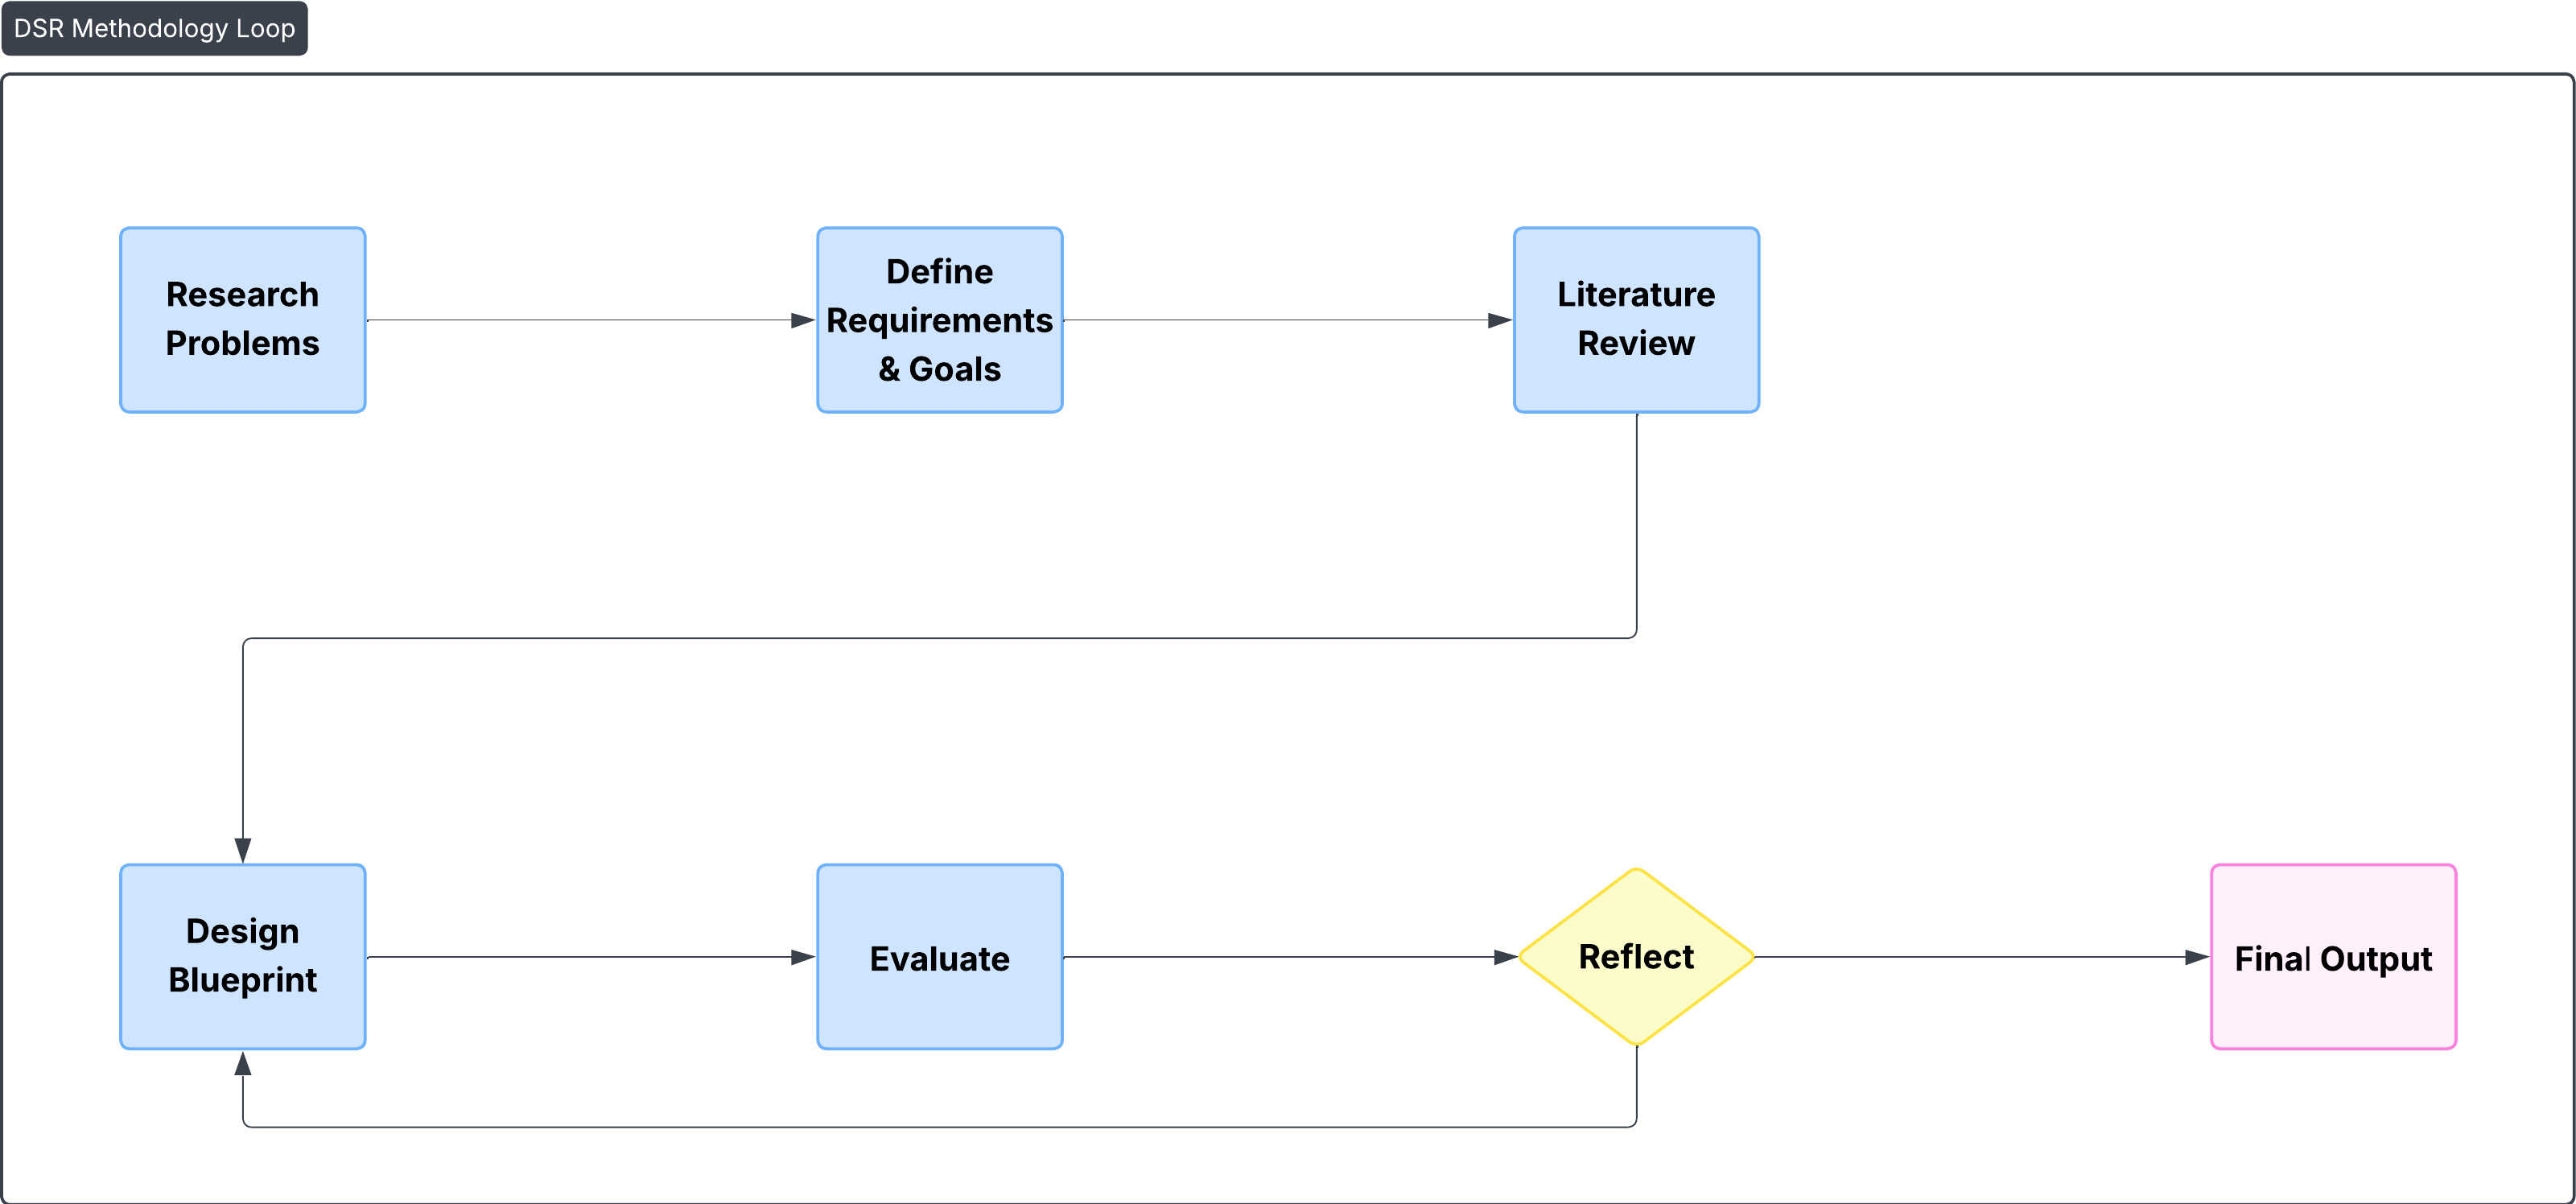
\includegraphics[width=\linewidth]{gfx/examples/dsr_loop.jpeg}
    \caption{Methodology: Design Science Research (DSR)}
    \label{fig:dsr-loop}
\end{figure}


\section{Problem Statement and Research Questions}
Organizations who want to build a ML classification solution, often lack the ability to develop and develop it. Success depends on the resources they allocate , which are frequently scarce, fragmented or poorly coordinated \cite{duda:2024}. Without a clear view on which resources matter the most , firms often misallocate effort and usually end up with costly , hard to reverse implementations.
When organizations finally move to implementation without enough upfront research , it is highly likely some unforeseen challenges might occur \cite{arpteg:2018}. During our literature review, we identified core challenges that recur across data and ML pipeline projects. To address them in a clear way , we are organizing the problems into two groups :

% --- Table 1: Foundational pipeline design ---
\begin{table}[htbp]
    \centering
    \begin{tabularx}{\linewidth}{@{}lX@{}}
        \toprule
        \textbf{\#} & \textbf{Problems in foundational pipeline design}                                                                                                   \\
        \midrule
        1           & Tight coupling : Updates in one component, causes a ripple effect that might break the whole system \cite{modi:2023}                                \\
        2           & Data Quality \& Governance: Inconsistent schemas and incorrectly defined data types lead to weak pipelines and unreliable models. \cite{foidl:2024} \\
        3           & Complexity: Modern MLOps tools are complex and costly for small companies. \cite{eken:2025}                                                         \\
        \bottomrule
    \end{tabularx}
    \caption{Problems in foundational pipeline design}
    \label{tab:problems_foundational}
\end{table}

% --- Table 2: Model lifecycle ---
\begin{table}[htbp]
    \centering
    \begin{tabularx}{\linewidth}{@{}lX@{}}
        \toprule
        \textbf{\#} & \textbf{Problems in model lifecycle}                                                                                                                                                                      \\
        \midrule
        1           & Versioning Data: There is no clear policy for versioning data , models and APIs which makes rolling back to a previously good state slow or impossible \cite{steidl:2023}.                                \\
        2           & Experiment tracking and reproducibility: Runs , datasets and model parameters are not tracked throughout model experiments, which causes unreliable evaluations and experiment results. \cite{idowu:2024} \\
        3           & Data drift: The production data gradually changes from what the model was trained on. Without retraining policies it can lead to performance decay on unseen data. \cite{cossu:202}                       \\
        \bottomrule
    \end{tabularx}
    \caption{Problems in the model lifecycle}
    \label{tab:problems_lifecycle}
\end{table}



Guided by the literature review and the problems we mentioned earlier, we define two research questions that shape the direction of the study.

\begin{enumerate}
    \item[\textbf{RQ1:}] \label{rq:1} What design principles enable a small team to build and operate a modular text-classification pipeline?
    \item[\textbf{RQ2:}] \label{rq:2} How can a text classification model maintain performance and accuracy under evolving data?
\end{enumerate}

\section{Scope of Work}
\subsection{Included in the scope}
\label{sec:scope}
This thesis seeks to deliver a reusable blueprint for a modular classification pipeline for small teams with limited resources. It specifies core pipeline stages of ETL (extract, transform , load), the interfaces needed to wire them, and a layered data layout for versioning datasets. The ML layer of the pipeline covers text-classification model selection as well as the steps for ingesting ,feature extraction ,  training ,evaluating  and serving the model. We will explore different retraining strategies along with their pros , cons and use cases in order to keep the model up to date with changing data. The blueprint will be validated through a realistic use case, which will demonstrate its applicability in practice.

\subsection{Out of scope}
\label{sec:out_of_scope}
This thesis does not compare alternative text-classification approaches or develop new ones. The focus is to design the end to end pipeline, where the developers can plug in their own text-classification model or approach. We do not deliver a production level codebase since this work is an architecture design derived from the literature review , not a deployable product. The implementation will be done in Python, using standard libraries without third-party frameworks. The design will not cover security programs, large scale optimizations , cloud deployment , unit and A/B testing or tasks beyond classifications.


\section{Use Case Overview: News Article Classification}
Use case overview
This thesis uses a realistic scenario from a real-world organization to derive the requirements and evaluate the end result. The organization’s business model centers around collecting data from different sources and later turning this data into business metrics for its clients. The development team consists of 3 developers and a CTO , which fits the limited resources use case for our thesis. The use case covered here is one component of their business model, which extends their current system. They plan to build a data warehouse that extracts relevant news from X/Twitter, transforms the content and later loads it into a database. On top of this . they want an ML classifier to categorize each news item with initially a single-label from known categories and later expand it to a multi-label classification for each news item. Because the pipeline will run periodically on daily intervals , the warehouse will have a continuous flow of new data that will be loaded into the warehouse. That's why the model must remain adaptable when new data arrives and not be affected by data drift. In addition the warehouse must preserve the original news text and keep transformations ,labels and predictions separate from the raw news. Results must be traceable to the exact inputs and parameters used for training and no step in the pipeline should overwrite raw data. The pipeline should run autonomously , be robust to errors and require minimal human intervention. Given the limited resources , before starting to implement this use case requires careful upfront architecture design. This scenario is well suited and represents an ideal setting to apply and evaluate the proposed modular classification pipeline

\section{Requirements Derivation}
From the problem statement and the industry use case , we can derive a set of general requirements for a modular classification pipeline with continual learning. These requirements abstract from recurring needs of different organizations so they remain use case agnostic and reusable. In the later sections , we will apply these general requirements for the news classification scenario and provide traceability from each requirement to the design decision we make.

% --- Table 1: Requirements overview ---
\begin{table}[htbp]
    \centering
    \begin{tabularx}{\linewidth}{@{}lXll@{}}
        \toprule
        \textbf{ID} & \textbf{Requirement}                                                                                  & \textbf{Category} & \textbf{Priority} \\
        \midrule
        R1          & Ingestion from data source. The pipeline must fetch and normalize data into a common staging area.    & Pipeline          & Must              \\
        R2          & Data integrity. Raw data immutable; transforms/predictions stored separately; never overwrite source. & Governance        & Must              \\
        R3          & Labeling of items. Single-label classification from known categories.                                 & ML                & Must              \\
        R4          & Traceability. All runs and predictions auditable to run, model version, and hyperparameters.          & Governance        & Must              \\
        R5          & Data quality. Schema and type validation before training/serving.                                     & Data Quality      & Must              \\
        R6          & Maintain accuracy as data evolves. System adapts to new data flow over time.                          & ML/CL             & Should            \\
        R7          & Minimal stack. Prefer simple libraries over third-party platforms (small team, limited resources).    & Arch/Cost         & Should            \\
        \bottomrule
    \end{tabularx}
    \caption{Requirements overview grouped by category and priority.}
    \label{tab:req_overview}
\end{table}

\chapter{Artifact Design - Components of a Modular Classification Pipeline}
\section{Overview}
\label{sec:overview}
In this chapter we deinfe all the components for an end-to-end text classification pipeline built on a robust ETL foundation, a layered data layout, and a lightweight ML layer with continuous learning. It specifies how raw data moves from diverse sources into a staging area, is transformed into reliable, queryable datasets, and is then used to train, evaluate, serve, and continually update a classifier without compromising data integrity or lineage.

\section{ETL Pipeline Design}

This section presents a clear ETL design for turning mixed source data into reliable, ready to use datasets. We begin with careful extraction guided by a simple data map and field level profiling so we pull only the fields we need without slowing source systems. Next, transformation cleans and standardizes the inputs, enforces schemas and types, handles missing values and duplicates, and logs any quality issues for later review. Finally, loading writes the results into partitioned, well defined tables, first with a one time backfill and then with regular incremental runs. The goal is a reproducible and traceable data that analytics and model training can trust. Here are the core components of the ETL design:

\subsection{Extraction}
The Extract-Transform-Load (ETL) begins with extraction. That means accessing one or more source systems to retrieve the data needed for downstream processing , and transferring it to a staging area \cite{mandala:2019} . The primary goal is to pull the required data with minimal impact on the sources, which means without degrading their performance response time or causing locks \cite{gjcs:2023}. Data sources can include transactional apps (CRM/ERP), APIs , files and IoT sensors. They can deliver data in different formats like :  relational tables, JSON , XML and logs. Data volumes may also vary widely depending on the business context.
\smallskip

That's why before building any extract job, define what to extract and why at a logical level. You can achieve this by producing a logical data map. A logical data map defines for each data field , their business meaning , original source and transformation rules \cite{kimball:2004}. After we have defined which data is necessary for the organization we list the systems and APIs likely to contain the required information. The next step after listing the sources that contain the required data , these data elements are then profiled in order to extract the necessary fields for the business need. Data in each source must be analyzed and each field must be profiled to determine its data type , unique identifiers , table relationships and cardinalities. As the final step of extraction , the pipeline determines which changes to pull from each source. After profiling , not every column is relevant , so the extractor should retrieve only the needed fields. The best query returns exactly what you need and not an entire table to be trimmed later \cite{kimball:2004}. In order to capture new or changed data we can query based on \texttt{updated\_at} field. The result of this stage is data with relevant fields selected and change rules defined and it's now ready for Transformation.
The ETL Pipline steps are shown in Figure~\ref{fig:etl_steps}.

\begin{figure}[htbp]
  \centering
  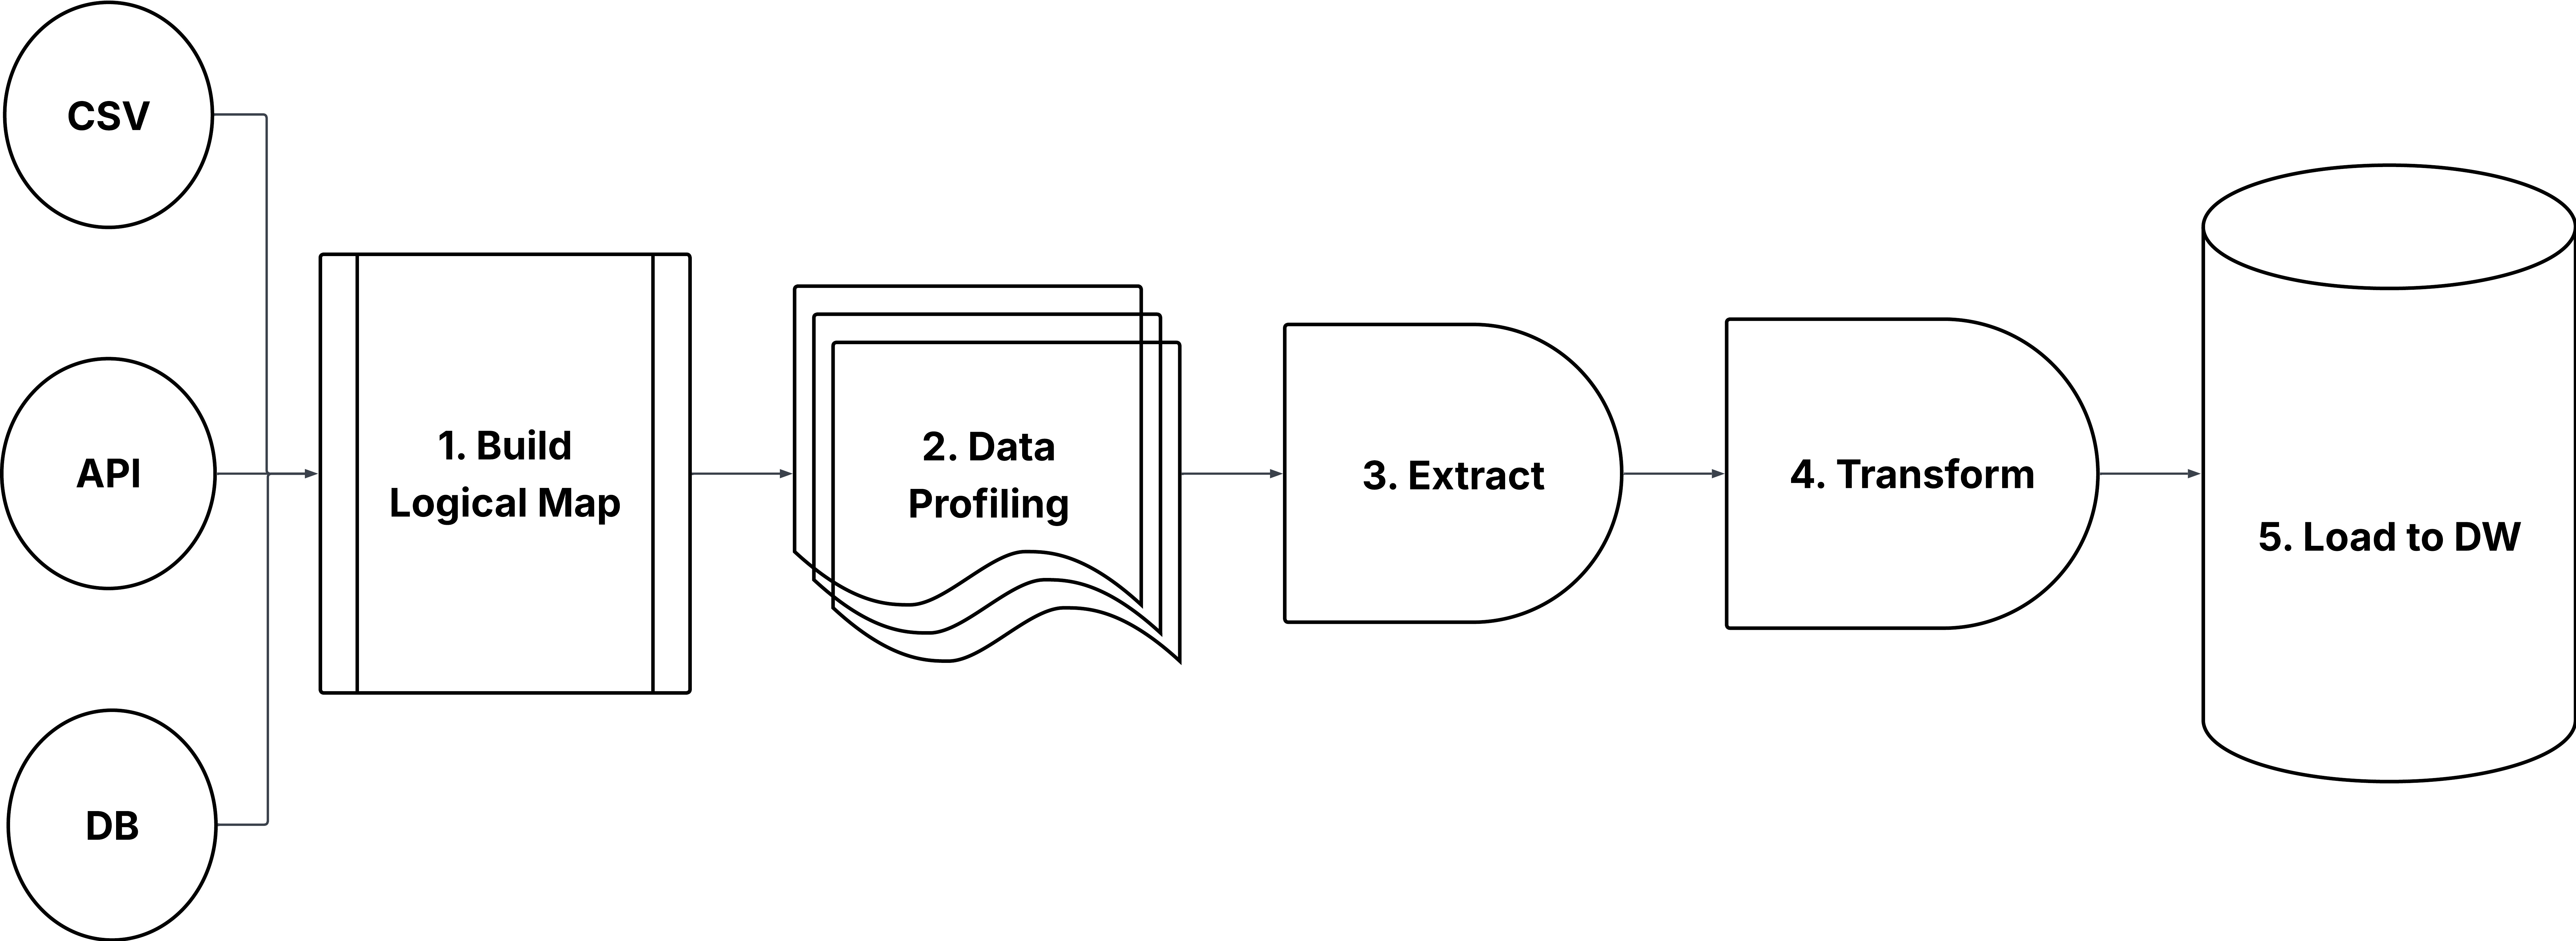
\includegraphics[width=0.8\linewidth]{gfx/examples/etl_steps.jpeg}
  \caption{ETL Pipline Steps.}
  \label{fig:etl_steps}
\end{figure}

\subsection{Transformation}
After extraction , data is standardized so it can be reliably stored and used for serving and modelling \cite{mandala:2019}. In practice , sources are heterogeneous (databases , files , APIs ) and formats vary, that's why a substantial part of analytics work is therefore pre-processing \cite{gjcs:2023} . Cleaning and conforming the data are ETL steps that add the most value , since they decide where the data is fit for purpose and produce metadata , like profiling results and error logs , that should travel with the data. These are the common steps that a transformation step should have \cite{bilal:2022}:

\paragraph{Standard Transformation Rules}
\begin{enumerate}
  \item[\textbf{1.}] \textbf{Standardise fields.} Normalise units like currencies, time zones, whitespaces, phone/email formats, and document any outliers.
  \item[\textbf{2.}] \textbf{Detect \& cast data types.} First infer base types, then re-scan the columns to classify them as native types.
  \item[\textbf{3.}] \textbf{Handle missing values.} Define your missing-values policy. Either leave them null, fill with the most frequent value, mark as ``unknown'', or drop the whole row.
  \item[\textbf{4.}] \textbf{Remove duplicates.} Drop exact duplicates and apply matching rules.
  \item[\textbf{5.}] \textbf{Detect outliers.} Flag extreme values where they would distort the ML model.
  \item[\textbf{6.}] \textbf{Apply calculations.} If the data field requires calculations, apply them before loading into the database.
  \item[\textbf{7.}] \textbf{Log events.} On any rule violation, write an error entry and attach an audit record to the metadata.
\end{enumerate}

\subsection{Loading}
\label{sec:load_patterns}
The loading step writes the transformed data into a central storage used for analytics and serving . In this blueprint , that means building datasets into the warehouse layers that later can be used for users and the ML models for training . Loading is where the pipeline turns intermediate files into queryable , partitioned tables with clear schemas , keys and partitions that jobs can rely on\cite{burgos:2022}. There are two load patterns that are most commonly used:



\begin{description}
  \item[The historical load.] This strategy backfills one or more tables with a large volume of past data, often months or years in a one-time load. This populates the warehouse with existing data before running daily jobs to extract new or changed data. In order to handle large volumes of data, the loading process is usually split into chunks to make it easier to load and less error prone. \cite{kimball:2004}

  \item[The incremental load.] After the first historical backfill, the pipeline switches to incremental loads, which adds new records and apply changes detected since the last run. Incremental behaviour can be append only or upsert (insert new or update existing), depending on the table's purpose. Append only is used for logs and immutable facts and is usually partitioned by date, while upsert is used for changing tables that require frequent updates. \cite{kamat:2022}
\end{description}

Whichever pattern is used , loads should be accurate and record where the data came from. A good load step is predictable and repeatable. Each run targets a known time window or partition and re-running produces the same result. For performance, large batches are written into the storage using bulk loaders and often in parallel by partition. \cite{kimball:2004}

With this behavior in place, the warehouse becomes a stable repository , ready to serve data for monitoring , analytics , training and business consumption.





\section{Data Warehouse Layer Design - Medallion architecture}
To keep the pipeline modular and make data accessible across each stage of transformation, we organize it into three logical layers. This “Medallion” pattern exposes data at each step of the transformation process, so producers and consumers of data will work against different interfaces instead of a single storage. Because of this architecture pattern , data quality improves at each layer. If a mistake occurs and some data is removed , we can always trace it back. In addition , this layered approach enables easier access control , so that different groups of people can be restricted to consume only specific layers \cite{wiselka:2024}. The result is a clear separation of concerns with simpler change management and better lineage of data.

\subsection{Bronze Layer}
Bronze Layer stores raw ingested data in its raw original format \cite{mohna:2022} . In this stage the raw data is stored along other ingestion metadata. This includes fields like \texttt{run\_id}, \texttt{ingest\_batch\_id}, \texttt{source}, \texttt{retrieved\_at}, and \texttt{unique\_identifier}. Loading strategy for bronze data is append only , that means once loaded into storage the data remains immutable. The data is typically partitioned by retrieved time or source that was extracted from \cite{gujjala:2024}. Because Bronze layer holds large volumes of raw data that we rarely directly read from , its main value that this layer adds is traceability and auditability. When needed , we can pull records from a specific day/week/monthor by source , making it easy to reconstruct past states without touching downstream layers \cite{gujjala:2024}. Minimal or no transformation happens during the bronze loading of data.

\subsection{Silver Layer}
The silver layer cleans and standardizes the captured raw data and turn them into tables ready to be used in analytics. At this stage , the pipeline enforces schema rules , cast types , fills in missing values , removes duplicates and applies semantic normalisation. It also performs essential data integration so that unstructured or semi-structured inputs become reliable and queryable formats \cite{nieto:2019}. Silver layer resolves data quality issues and prepares conformed datasets for downstream loading and modelling. It presents a consumption focused view that may power real-time dashboard or predictive services

\subsection{Gold Layer}
The gold layer delivers curated datasets for Business Intelligence (BI) dashboards and Ai applications \cite{garagnani:2013}. It holds use case specific tables built by selecting tables from earlier layers or sources and applies aggregations and business rules \cite{wiselka:2024}. All analytics and calculations happen in Gold layer, so upstream SIlver and Bronze remain untouched, preserving original data and lineage. Gold tables can also carry model outputs and monitoring attributes. For example, a \texttt{predictions} table can store the predicted result together with model metadata, like \texttt{model\_version}, \texttt{model\_type}, \texttt{used\_hyperparameters}, \texttt{run\_id} and \texttt{predicted\_at} to link each prediction to the corresponding silver record via its \texttt{unique\_id}. This create a Gold association table that stores predictions without modifying Silver data, preserving immutability and prevents corruption of data. This separation keeps ML logic distinct from business view while delivering first-class, consumption-read data to users.
Here is a visual representation of the Medallion architecture in Figure~\ref{fig:medallion}.

\begin{figure}[htbp]
  \centering
  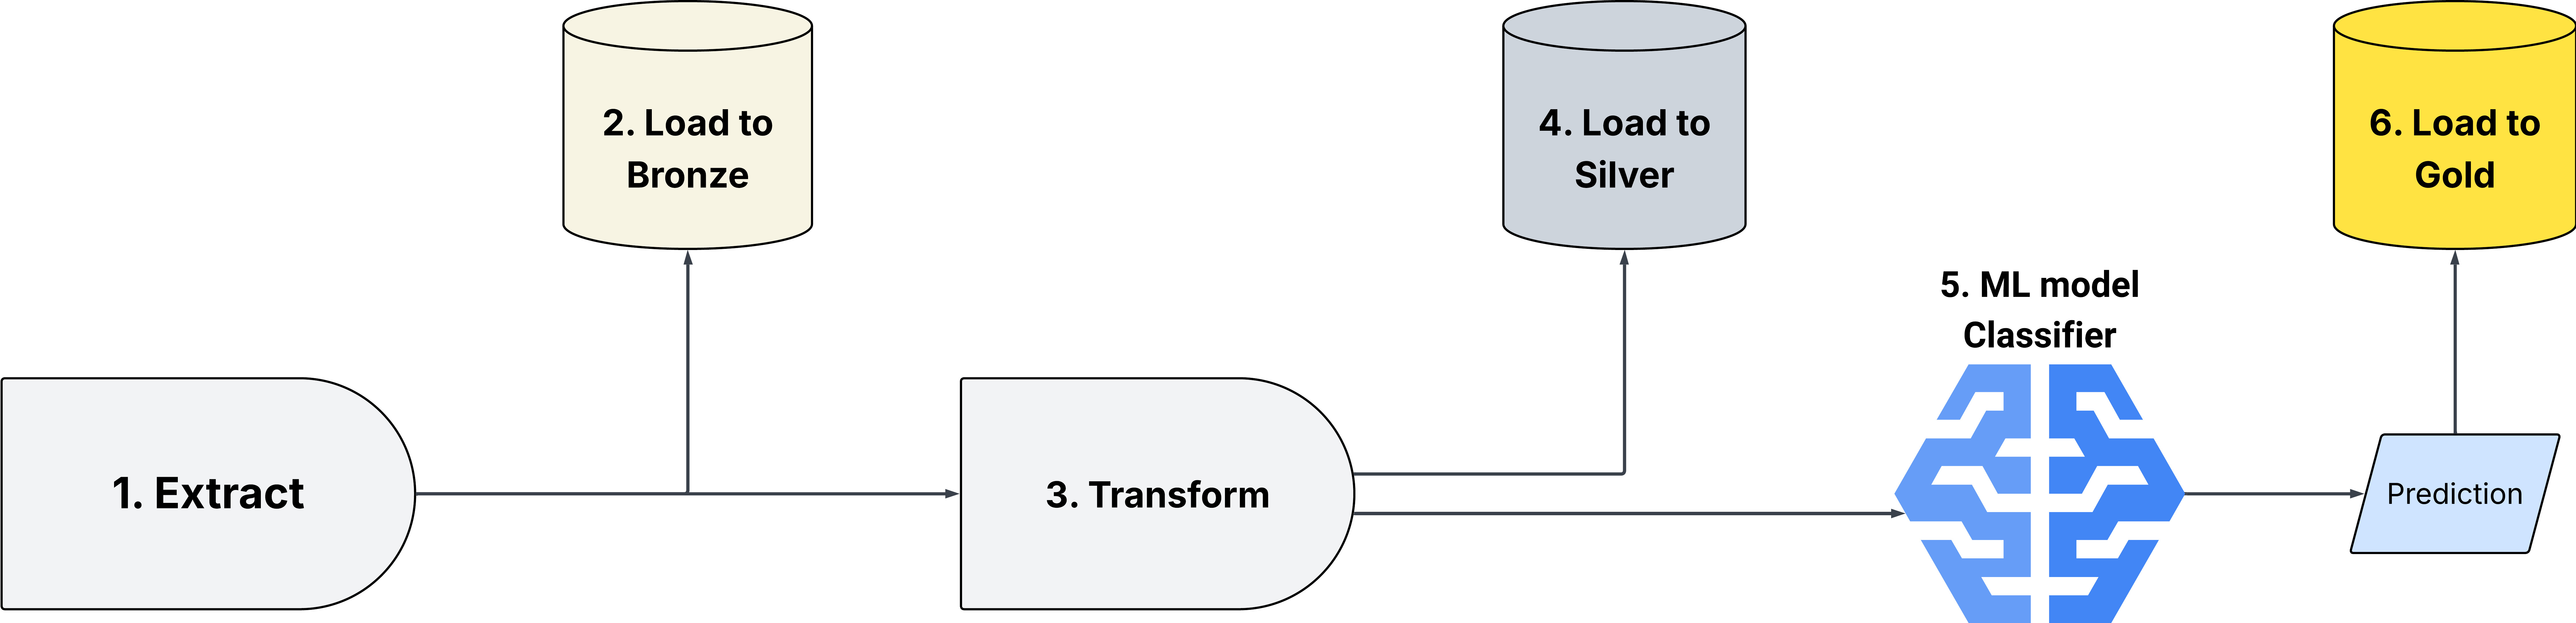
\includegraphics[width=\linewidth]{gfx/examples/medallion.jpeg}
  \caption{Extended ETL Pipeline with Medallion Architecture.}
  \label{fig:medallion}
\end{figure}

\section{ML Layer Design }
Text classification is a core task in Natural Language Processing (NLP) and data mining. It uses machine learning to assign predefined labels to documents so that it provides more context to the text and makes it easier to filter and analyze \cite{allam:2024}.
\smallskip

In the context of this thesis we will frame text classification as supervised machine learning with single-label classification, where the model is trained on a dataset with predefined categories and learns relationships between input and their labels. Afterwards it uses the learned mapping to assign categories or labels to new, unseen texts \cite{wang:2023}.
\smallskip


This module will upgrade the modular ETL pipeline into a full classification pipeline by integrating  ML processes into it. This sub-module is inserted between the silver layer and gold layer, where we use the silver data and perform ML tasks on them.


\subsection{Text classification processes}
Below is a concise overview of all the different stages that the texts goes through before being label. Text classification in practice is not a single model but an evolving process that must keep up with changing data and business goals. Treating it as a set of modular processes helps small teams to upgrade or change one process without disturbing the rest. Here are the key stages the text passes through in our classification pipeline \cite{daud:2023},from clean Silver input to validated predictions logged in Gold.

\begin{enumerate}
  \item Preprocessing
  \item Train/Test Split
  \item Feature Extraction
  \item Model Selection \& Training
  \item Evaluation
  \item Serving
\end{enumerate}

\subsubsection{Preprocessing}
The preprocessing stage cleans and organizes the dataset so it is suitable for classification. Its goal is to reduce noise and inconsistencies and to produce a stable input for the model. The outcome is a structured , conformed dataset that can be safely passed to the training stages. The pre-processing steps performed are defined in here:

\paragraph{Dataset Structuring and Balancing}

\smallskip
In this step we consolidate the textual fields into a single input column. That means if multiple text attributes like for example a news article that has a headline , author and text we merge them into one text. We als standardise labels that may have been written in acronyms or abbreviations into full words.
\smallskip

To address class imbalance, categories which come rarely into the dataset are excluded from modelling. Also from the remaining classes we balance them by reducing the amount of samples to match the size of the smallest represented class \cite{daud:2023}. We record each class counts before and after balancing and visualise distributions to verify the final dataset is suitable for fai evaluation.

\paragraph{Label Encoding}

\smallskip

For modelling task , category labels must be numeric. We apply label encoding to map each distinct class name to an integer id \cite{ahmed:2021}. The resulting integer codes replace the original text labels only in the training data. We persist the mapping of class name to integer with the run metadata so predictions can be decoded back to text labels and experiments are reproducible


\paragraph{Data Preprocessing \& Tokenizing}

\smallskip

We prepare the raw text with a small preprocessing routine so the model sees clean inputs. First, we lowercase all characters so meaning does not depend on letter case. We then remove special characters and digits and normalize whitespaces to single spaces. Next we strip stopwords using a standard list so very common function words do not dominate the representation. Finally we tokenize the text into individual terms and apply light stemming step , so variants like go and going map to a common root. The result is a structured sequence of normalized tokens suitable for downstream feature extraction.


\subsubsection{Train/Test Split}
After feature extraction is defined , we split the dataset into training and test sets to get an unbiased estimate. We use here a 70/30 split where 70\% of data is used for training and 30\% for testing.  We fit the TF-IDF vectorizer on the training dataset only.

\subsubsection{Feature Extraction}
Machine learning models operate on numeric representations, not raw text. Therefore, tokens must be converted into vectors before training. In this study, we use Term Frequency–Inverse Document Frequency (TF-IDF), which is effective for text categorization when word order is less critica \cite{das:2023}. TF-IDF uses two measures:

\begin{itemize}
  \item \textbf{Term Frequency (TF) } how often a term appears in a single document
  \item \textbf{Inverse Document Frequency (IDF): } shows in how many documents a word appears , across the entire dataset

\end{itemize}

\smallskip
We first build a fixed vocabulary from the training data and fit the TF-IDF vectorizer, learning the vocabulary and IDF weights. Each term is assigned a column in the feature space, and each document becomes a row where most entries are zero and the non-zero entries are that document’s TF-IDF weights for the terms present \cite{das:2023}. The fitted vectorizer is then reused to transform validation, test, and future prediction data so the same mapping applies consistently.

\smallskip

Combining TF and IDF balances term importance,where very common words receive lower weights, while more distinctive words receive higher weights. This prevents frequent but less meaningful terms from dominating the model.

\smallskip

After feature extraction, we obtain a sparse TF-IDF document–term matrix with one row per document, the encoded label vector, and the fitted vectorizer containing the vocabulary and IDF weights needed to transform future text into the same feature space.

\subsubsection{Model Selection \& Training}
The pipeline keeps model choice flexible as it accepts any classifier that respects the input-output contract. Based on our literature review we have compiled a list of traditional ML models that can be used for different classification tasks  \cite{allam:2024} :

\begin{table}[htbp]
  \centering
  \begin{tabularx}{\linewidth}{@{}lX@{}}
    \toprule
    \textbf{Model}            & \textbf{Evaluation}                                                                  \\
    \midrule
    Logistic Regresion        & Strong baseline for TF-IDF , fast , interpretable and well-calibrated                \\
    Linear SVM                & Excels on high-dimensional sparse text                                               \\
    Naive Bayes               & Very fast and simple. Works well with word counts.                                   \\
    Random Forest             & Less common for sparse TF-IDF, works better for dense features.                      \\
    K-nearest Neighbors (KNN) & simple and instance based. Works well for small datasets but is slower at interface. \\
    RNN                       & with this model representation of a word depends on the sequence of the tokens.      \\
    Transformers (e.g.\ BERT) & Contextual embeddings. Heavy, but offer the best performance.                        \\
    \bottomrule
  \end{tabularx}
  \caption{Text classification model options .}
  \label{tab:text_cls_models}
\end{table}

After the model of choice was decided we proceed to train it with our chosen dataset. We train models in a simple and repeatable manner. We use the fitted TF-IDF vectorizer to transform training and test data into TF-IDF matrices \cite{daud:2023}. Afterwards it's time to choose the hyperparameters. They control how a model learns and how complex it is \cite{ilemobayo:20243} . Each model has a different set of parameters settings , which we chose before training. Adjusting these values to the given features improve efficiency and accuracy of the model. The process of searching for and selecting the best settings is called hyperparameter tuning \cite{daud:2023}. The last step would be to load the model in a model registry , in the cloud or locally in order to use its prediction function. Now the model is ready for serving and the outcome of this stage is a trained model on a custom dataset ready to be evaluated.


\subsection{Evaluation}
After training the selected classifier , we assess its performance on a series of test metrics. These metrics are used to evaluate the model effectiveness in classifying text with the according label \cite{allam:2024} :

\begin{description}
  \item[Accuracy] measures the share of all predictions that are correct. It is simple and widely used , but can be misleading when classes are imbalanced.
  \item[Precision] measures how many predicted positives are truly positive. It quantifies the purity of positive predictions.
  \item[Recall] measures how many of the actual positives the model correctly identifies. High recall means few missed positives.
  \item[F1-Score] measures the harmonic mean of precision and recall , providing a single score that balances both error types. It is useful with uneven class distribution or when false positives and false negatives both matter.
\end{description}

Taken together all the evaluation metrics provide a view of how well the selected classifier assigns corrects labels. These metrics form the basis for comparing variants of the model.
To connect the results of prediction and evaluation metrics with the data , we write both of them into a predictions table with , \texttt{document\_id}, \texttt{model\_version} , \texttt{hyperparameters}, \texttt{run\_id} and \texttt{predicted\_at}. Because \texttt{document\_id} also exists in Silver layer , we can join predictions with the Silver data to form the Gold data. This keeps raw and cleaned data immutable and enables straightforward comparison across model variants.


\subsection{Serving}
er model training , we expose the model inference in order to communicate with our other system.TensorFlow, a widely used library in the ML ecosystem, is needed for a modular serving system. We separate concerns of  model lifecycle management from the inference execution in order to have a clear modular interface \cite{ilemobayo:20243}:


\begin{description}
  \item[Inference execution] measures the share of all predictions that are correct. It is simple and widely used , but can be misleading when classes are imbalanced.
  \item[Model lifecycle management] measures how many predicted positives are truly positive. It quantifies the purity of positive predictions.
\end{description}

\section{Continuous Learning}

When data distribution shifts over time , static models lose performance. Neural Models trained once on a fixed dataset tend to forget past patterns or overfit to fresh patterns when updated naively. This is called “catastrophic forgetting” \cite{chrysakis:2020}. In order to solve this we need to retrain the model with specific strategy in order to maintain performance as new data comes in. This is an extension of our pipeline which handles pretty advanced topics and the research on this is pretty new , so we will be introducing here today some strategies that can help to continuously feed knowledge to our ML models.
\smallskip

The goal of this section is to design a framework for continuous learning that keeps a ML classifier reliable and performant as data distributions evolve. Concretely we aim to detect performance drift , decide which strategies we should use to retrain the model and set scheduling triggers for retraining. By defining this steps inside the data classification pipeline, we maintain accuracy on our predictions for new data and ensure the system learns from fresh data without forgetting prior knowledge.

\subsection{Detecting data \& performance drift}
We set up parallel monitoring items in order to detect both the data drift from input data and performance drift from prediction outputs.

\paragraph{Detecting Data Drift}
We maintain summaries of each feature and routinely compare recent time windows to a fixed reference set using tests like Population Stability Index (PSI) or KL divergence \cite{cossu:202}. This gives us early warning signals , to measure how far the current feature distribution has moved from the referenced data . We enforce schema and data quality guards like valid ranges or category frequencies to detect pipeline faults. This are needed to detect distribution shifts before they degrade accuracy and provide auditable evidence when and why retraining is needed.

\paragraph{Detecting Performance Drift}
Before learning from new labels,we perform a prequential task , which tests the performance of the next batch before training the mode \cite{cossu:202}. We track common metrics like overall accuracy. We do this not only for the whole batch but for segments of the batch as well to test accuracy on different groups inside the new batch to see if new data , that our model can’t confidently and accurately  predict, exists. With this monitoring items we localize failures in a batch of data and distinguish brief noise from continuous performance degradation.


With data and performance drift monitored we defiance explicit thresholds and log every alert , so that we notice drift signals and make them actionable, to ensure retraining is justified.


\subsection {Retraining strategies}
With our layered data and monitoring in place, we can now select a continuous learning strategy to keep the model robust under data drift. Before choosing , we should define clear objectives, like , target KPIs and metrics , acceptable latency and costs and governance rules for storing historical data. Each strategy group have distinct trade offs in resources , risk and complexity, that’s why we outline the main options in this section [61] :


\subsubsection*{Regularization based}
\begin{description}
  \item[Description] We keep a frozen copy of the last good model as a teacher and while training the new model on new fresh data we add constraints so that its parameters do not drift too far away from the old model’s behavior. We implement a weight regularization function that penalizes the new model if there are big changes in weights.
  \item[Pros] We can retrain frequently because we only need a frozen teacher model in our current training loop which adds small loss. This works as well if we don't want to store historical data , since knowledge distillation can be done on new batches from our teacher model. This produces stable updates with clear auditability because the new model is explicitly tied to the previous one.
  \item[Cons] Can adapt too slowly under hard distribution shifts. Performance is sensitive to hyperparameters like penalty on weight and temperature. If the teacher has errors or biases , the student may inherit them.
  \item[When to use] When we want the simplest safe baseline before adding more complexity to the continuous learning. Useful for frequent , small updates where stability is more important than trying to improve little amounts of accuracy.
\end{description}

\subsubsection*{Replay-based}
\begin{description}
  \item[Description] Replay-based continual learning fights forgetting by rehearsing a small , representative slice of past data , while learning from new data. When we build retraining batches we keep a distribution of 60\% new data and 40\% old data. After each cycle , we refresh the distribution by inserting the most representative newly labeled examples and removing redundant oldest ones. This keeps the class balanced and guard against overfitting.
  \item[Pros] Very efficient against catastrophic forgetting by directly rehearsing on old knowledge. Flexible variants exist if we want to optimize the strategy by changing the distribution of old/new data or other parameters.
  \item[Cons] Needs to be configured on what data to keep and how much. Multiple replays adds training and maintenance overhead and may suffer from quality issues if the data chosen to retrain is not representative.
  \item[When to use] When we care about maximizing accuracy over time when new data comes in this is the best strategy to use. Also when we see that data drift is high and have enough control over data governance then this is a great default for production pipelines once we implement basic data handling policies.
\end{description}

\subsubsection*{Optimization-based}
\begin{description}
  \item[Description] In this method we reduce forgetting by changing how we update the weights, not the model itself. We keep a class-balanced old dataset that represents past knowledge. During each training for each batch of new data we compute a signal if that would harm old performance. If it does we reshape the update so it doesn’t increase old loss.
  \item[Pros] Gives more control over learning so that new learning does not harm old behavior. It can be layered on top of other retraining strategies like replay-based to optimize the model more without changing architecture
  \item[Cons] More compute overhead. Sensitive to implementation details, batching and randomness.
  \item[When to use] We have enough gpu resources and an experienced team.
\end{description}

\subsubsection*{Representation-based}
\begin{description}
  \item[Description] This strategy relies on stable features instead of constantly changing the whole architecture. We use a pre trained encoder and freeze most of the weights. Than learn only small parts like the classifier head , adapters or prompts so the backbone changes little and the representation space stays consistent.  We maintain a class prototype , which is the mean feature per class and use them for calibration or quick checks that the space hasn’t drifted.
  \item[Pros] Fast and low risk updates by relying on stable pretrained encoders and training only a small part of the classifier. Excellent fit for frequent retrains with limited compute power.
  \item[Cons] If the fixed encoder is too frozen , performance can degrade under large data drift.
  \item[When to use] Quick and low-cost updates like weekly or daily scheduling. We already have strong pretrained text encoders and want minimal risk to production.
\end{description}



\chapter{Aplying the Case Study \&- Conclusion}
\label{ch:conclusion}
This chapter shows how the proposed pipeline is applied to the industry-inspired scenario where a small team builds a warehouse and classifier for X/Twitter news. We follow the blueprint step by step and make concrete design choices that fit the team needs.
We also draw the main conclusions of the thesis.


\section{Case Study: News Classification on X/Twitter}

\subsection{Extraction Strategy , Transformation Schema and Loading}

We extract news from X/Twitter using the Recent Search endpoint, which returns public posts from the last week with a simple authenticated request, for example:
% preamble: \usepackage{listings}
\begin{lstlisting}[language=bash,caption={Recent search via X API},label={lst:x-recent-search}]
curl --request GET \
  --url https://api.x.com/2/tweets/search/recent \
  --header 'Authorization: Bearer <token>'
\end{lstlisting}

Before writing any extractor, we define a logical data map that lists each field we will store, its meaning, and how it will be used downstream.

% Requires in preamble:
% \usepackage{tabularx}
% \usepackage{booktabs}

\begin{table}[htbp]
    \centering
    \begin{tabularx}{\linewidth}{@{}l l X X@{}}
        \toprule
        \textbf{Field}  & \textbf{Type}   & \textbf{Meaning}                                         & \textbf{How is used}                                                            \\
        \midrule
        id              & string          & Unique identifier of the post                            & Primary key, deduplication, stable join key across layers                       \\
        created\_at     & timestamp (UTC) & Time the post was created                                & Event time for partitions and time series analysis, windowed metrics, backfills \\
        author\_id      & string          & Stable identifier of the author                          & Join to user table, author level features, longitudinal analysis                \\
        username        & string          & Public handle of the author                              & Display in UI, secondary dedup checks, moderation workflows                     \\
        text            & string          & Full text of the post                                    & Main model input, search index content, text preprocessing and tokenization     \\
        public\_metrics & integer         & Number of likes                                          & Feature engineering, sampling strategies, evaluation  by engagement             \\

        retrieved\_at   & timestamp (UTC) & Ingestion time recorded by our pipeline                  & Lineage, Bronze partitioning, reproducible re-runs and auditing                 \\
        source          & string (enum)   & Provenance label, for example \texttt{x\_recent\_search} & Data lineage and filtering when multiple sources are combined                   \\
        \bottomrule
    \end{tabularx}
    \caption{Logical data map: fields, types, meaning, and downstream use.}
    \label{tab:logical_data_map}
\end{table}

Afterwards  we conduct field profiling that validates what arrives matches our expectations and is worth keeping. Concretely, we check data types and formats for \texttt{id} and \texttt{created\_at}, completeness rates for \texttt{text}, uniqueness of \texttt{id}, and consistency of \texttt{author\_id} to catch orphaned records. On the content side, we measure basic text characteristics such as length, presence of URLs, mentions, and hashtags, and run a lightweight language detection to ensure we ingest the intended language. For \texttt{public\_metrics}, we verify nonnegative integers and flag extreme values for review. These profiling steps help us trim unused attributes, document assumptions, and detect source quirks early. The extractor returns only the mapped fields, along with minimal ingestion metadata like \texttt{retrieved\_at} and \texttt{source}, and prepares them to be written into staging area. This keeps the footprint on the source small, reduces downstream cleaning, and gives us a well described, analysis ready subset of the stream.

\FloatBarrier

\subsection{Medallion layout}

\paragraph{Bronze}
Bronze stores the raw API payloads exactly as received from the Recent Search endpoint, together with minimal ingestion metadata such as \texttt{run\_id}, \texttt{ingest\_batch\_id}, \texttt{source}, \texttt{retrieved\_at}, \texttt{connector}, \texttt{version}, and \texttt{http\_status}. Data is written append-only and partitioned by \texttt{retrieved\_date} and \texttt{source}. The table \texttt{bronze.tweets\_raw} keeps the native \texttt{id} field but applies no transformations. This layer is the legal record of what arrived and when, which preserves originals for audit and allows any past day to be reprocessed.
\paragraph{Silver}
Silver standardizes structure and quality for analysis and modeling. Only rows that pass basic checks are promoted from Bronze: valid JSON, required fields present (\texttt{id}, \texttt{created\_at}, \texttt{author\_id}, \texttt{text}), parseable timestamps, nonnegative metrics, and no duplicates by \texttt{id} within the partition. At this stage we cast types, deduplicate by \texttt{id}, drop rows with null \texttt{text} or invalid timestamps, and apply light normalization while keeping an untouched copy of the text as \texttt{text\_raw}. We also derive simple flags such as \texttt{lang}, \texttt{has\_url}, \texttt{has\_hashtag}, \texttt{has\_mention}, and \texttt{text\_len}, and ensure \texttt{created\_at} is not after \texttt{retrieved\_at}. The main table, \texttt{silver.tweets\_clean}, includes \texttt{document\_id} (alias of \texttt{id}), \texttt{created\_at}, \texttt{author\_id}, \texttt{username}, text\_raw, \texttt{text\_clean}, \texttt{public\_metrics}, the derived flags, \texttt{retrieved\_at}, \texttt{source}, and a \texttt{bronze\_run\_id} pointer. Partitioning can use \texttt{created\_date} for analysis or \texttt{retrieved\_date} for operational symmetry.
\paragraph{Gold}
Gold provides curated views for business use and records ML outputs without changing upstream data. A curated table, \texttt{gold.news\_curated}, associates selected columns from \texttt{silver.tweets\_clean} and applies any documented business filters, for example language or moderation rules. Predictions are stored in \texttt{gold.predictions}, with one row per inference and columns for \texttt{document\_id}, silver snapshot or hash, scoring \texttt{run\_id}, , optional scores,predicted\_label, \texttt{predicted\_at}, and full model lineage such as \texttt{model\_version}, \texttt{model\_type}, \texttt{used\_hyperparameters}, \texttt{training\_run\_id}, and the training data window. Typical usage joins \texttt{gold.news\_curated} with the latest prediction per \texttt{document\_id} to serve labeled content, or starts from \texttt{gold.predictions} and joins back to \texttt{silver.tweets\_clean} and if needed to Bronze to audit via bronze\_run\_id any individual result. This separation keeps history across model versions, supports reproducible comparisons, and ensures upstream layers remain immutable.

\subsection{Loading Strategy}
We start with a historical backfill to populate Bronze and Silver,and split into manageable chunks. After that, we switch to daily incremental loads. Append only is used for immutable facts in bronze, while upsert is used where corrections are expected like silver. Each run targets a known partition and is repeatable. Bulk loading by partition gives predictable performance.


\subsubsection{Model Choice , training and evaluation}
For the first single label version we use a Linear SVM with TF-IDF features. We fit a TF-IDF vectorizer on the training split, persist its vocabulary, and transform validation and test with the same mapping. We tune the regularization parameter C and the maximum number of features for TF-IDF with a small grid search and stratified k-fold cross validation  We also set class weights to balanced when the label distribution is skewed. All artifacts that affect inference are versioned, the label encoder, the fitted TF-IDF vectorizer, and the SVM weights.

\smallbreak
Evaluation follows a simple, repeatable protocol.We use a consistent data splitting approach that preserves label balance and supports fair, repeatable evaluation. On the test set we compute accuracy,  precision,  recall, and  F1, and we include per class evaluation to study minority class behavior.
Every training run writes a compact run record with \texttt{run\_id}, \texttt{model\_version}, \texttt{model\_type}, \texttt{hyperparameters}, \texttt{tfidf\_config}, \texttt{feature\_spec\_version}, random\_seed, and the exact \texttt{silver\_snapshot\_id} or \texttt{silver\_snapshot\_hash} used for training.
\smallbreak



After trainging, we log results into Gold. The table \texttt{gold.predictions} stores one row per inference with \texttt{document\_id}, predicted\_label, optional \texttt{score} or \texttt{probability}, \texttt{predicted\_at}, \texttt{model\_version}, \texttt{training\_run\_id}, and a pointer to the Silver snapshot. This table never mutates Silver and allows us to retrieve the exact input later. Aggregate metrics go to \texttt{gold.eval\_daily} and \texttt{gold.eval\_by\_class}. The daily table holds \texttt{date}, \texttt{metric\_name}, metric\_value, \texttt{model\_version}, \texttt{run\_id}, and the data window used. The by class table adds \texttt{class\_name} and supports dashboards that track macro and per class trends over time. With these two Gold outputs we can serve labeled news to users and audit model quality by date, class, and \texttt{model\_version} without changing the upstream layers. When we later upgrade to multi label, the same contracts hold: predictions become arrays or a sparse label set, scores become per label vectors, and the evaluation tables add micro and macro averages for multi label without any change to the ETL or layer boundaries.

\subsubsection{Monitoring \&Retraining Strategy}

News streams shift quickly. Topics, entities, and wording change week to week, but yesterday’s knowledge still matters. A naive retrain on only the newest data adapts fast but forgets earlier patterns, which shows up as swings in per class performance. Replay based learning mixes a slice of past labeled examples with the latest labels, so the model rehearses what it already knows while learning new topics. This is a good match for short texts with fast vocabulary churn, limited labeling capacity, and a small team, because it is simple to operate, stable across updates, and compute friendly
\smallbreak

First We track two kinds of drift. First, input drift from the data we fetch,where for each key feature we keep rolling summaries over a recent time window and compare them to a fixed reference window. For text, this includes token frequencies, average text length, share of posts with links, mentions, or hashtags, and language share. For numeric fields like engagement counts we check basic moments and rate distributions. We set clear thresholds, and alert when a feature moves beyond its constrain. Second, performance drift from the model,where on the next incoming batch with labels available, we run a prequential check that scores the batch before training and records accuracy,  precision,  recall,  F1, and per class metrics. Both input and performance monitors write dated records to Gold so we can review trends by date, segment, and model version.

\smallbreak

We implement replay in a simple, repeatable way. First, we maintain a class balanced pool of past labeled news together with their labels and basic lineage, stored as a small table (for example \texttt{gold.retraining\_pool}) with fields like \texttt{document\_id}, \texttt{label}, \texttt{inserted\_at}, and a \texttt{selection\_score}. After each cycle, we refresh this pool by adding a small, representative sample from the newest labeled data and removing redundant or least informative items, so the pool stays within a fixed size and rare classes remain present. When retraining is triggered, we build the training set by mixing recent labeled data with a replay slice from the pool, and we pin all inputs to a stable snapshot so they are reproducible. We then train under the existing input and output contracts, tweak key hyperparameters and validate  from the same window. Next, we log run metadata, metrics, and candidate predictions to dedicated evaluation and prediction tables, and we compare the candidate against the active model on the same time ranges. If the candidate meets acceptance thresholds overall and on critical classes, we promote it by updating the production model in the model registry. This keeps the process clear, auditable, and low effort for a small team.



\section{Requirement Mapping}
This section explains how our implemented pipeline satisfies each requirement by mapping it to specific design choices and pointing to concrete artifacts in the thesis.
% Requires in preamble:
% \usepackage{tabularx,booktabs}
% \newcolumntype{Y}{>{\raggedright\arraybackslash}X}

\begin{table}[tbp]
    \centering
    \footnotesize
    \begin{tabularx}{\linewidth}{@{}l l Y Y Y@{}}
        \toprule
        \textbf{ID} & \textbf{Type}     & \textbf{Requirement}                                                                     & \textbf{Design choice}                                  & \textbf{How applied in case study}                                                                                                  \\
        \midrule
        R1          & Pipeline Must     & Fetch and normalize data into a common staging area                                      & Logical data map and low impact extraction into staging & Use Recent Search API, select mapped fields only, add retrieved\_at and source, land to Bronze staging                              \\
        R2          & Governance Must   & Raw data immutable; transforms and predictions stored separately; never overwrite source & Medallion layout and append only Bronze                 & Bronze keeps raw payloads immutable; Silver holds cleaned data; predictions recorded in Gold without altering upstream              \\
        R3          & ML Must           & Single label classification from known categories                                        & Linear SVM over TF IDF with label encoder               & Train single label classifier now; keep interfaces so multi label can be added later without changing ETL                           \\
        R4          & Governance Must   & Runs and predictions auditable to run, model version, and hyperparameters                & Full lineage logging and model registry                 & Log run\_id, model\_version, model\_type, used\_hyperparameters, silver\_snapshot\_id; store predictions with predicted\_at in Gold \\
        R5          & Data Quality Must & Schema and type validation before training or serving                                    & Promotion gates at Silver                               & Enforce required fields, types, dedup by id, basic text normalization; only passing rows promoted to Silver for ML                  \\
        R6          & ML/CL Should      & Adapt to new data flow as it evolves                                                     & Drift monitoring plus replay based retraining           & Track input and performance drift; on threshold, retrain with mixed new and replay items; log eval in Gold and promote via registry \\
        R7          & Arch/Cost Should  & Prefer simple libraries over heavy third party platforms                                 & Minimal stack with clear contracts                      & Python jobs, TF IDF, Linear SVM, small model registry, RPC predict endpoint; decoupled layers via stable schemas                    \\
        \bottomrule
    \end{tabularx}
    \caption{Requirement rewrite and mapping to design choices and their application.}
    \label{tab:req_mapping_rewrite}
\end{table}
\FloatBarrier
\section{Conclusion}
This thesis designed and validated a modular classification pipeline with embedded continuous learning for small teams with limited resources. By decoupling our pipeline into multiple components that interact with each other like: ingestion, transformation, loading, modeling, evaluation, serving, and monitoring through clear interfaces and data contracts, the blueprint reduces complexity, supports safe change, and preserves lineage across the full lifecycle. The news case study showed how the architecture turns into concrete choices. Every run is auditable and Raw data stays immutable.

The blueprint helps companies move faster from raw data to decisions while keeping risk in check. The staged layout (Bronze, Silver, Gold) makes quality and governance tangible, where raw inputs stay immutable, cleaned datasets are standardized for analytics, and predictions plus metrics are recorded without mutating upstream layers. This separation of concerns improves reliability and enables reproducible rollbacks, which is especially important when requirements evolve. The outputs in Gold are immediately consumable by dashboards and services, while model lineage and run metadata support audits and stakeholder trust.
\smallbreak

The design follows up to date data platform practice. It uses layered datasets, quality gates, experiment tracking, and a clean model training . What makes this design powerful are these three built in traits:

\begin{itemize}
    \item \textbf{Traceability:} every result is explainable over time, every experiment tracked and each data stage versioned.
    \item \textbf{Adaptability:} monitored drift triggers a repeatable retraining loop that keeps the models adaptable to new data distributions..
    \item \textbf{Composability:} pipeline is build on different modules that can be upgrade independently, so new extractors, models, or retraining strategies can be plugged in without changing the whole system.
\end{itemize}

\subsection{Limitations}
There are some limitations to this work. First, this thesis is a design blueprint. It offers a high-level architecture, not a full product. Each module can be implemented, but doing so needs more example work, patterns, and tests. Teams will need to study concrete cases for their domain before coding. The case study is a simplified scenario that does not cover all real world complexities. For example, it assumes clean labels are available for retraining, which may not hold in practice. On a technical level , the pipeline does not address streaming instead it focuses on backills and daily batches. Also there is no deplyoyment automation or infra as code, which are important for production. Finally, the blueprint does not cover advanced topics like data privacy, security, or compliance, which are critical in many industries.

\subsection{Future Work}
Future work can extend this blueprint in several ways. We can turn the blueprint into a reference implementation with code examples, tests, and deployment guides,which  would help teams get started faster. WE can upgrade some core components , like introducing streaming ingestion and real time scoring, which would make the pipeline more responsive. We can also explore more mmonitoring and retraining strategies, like active learning or semi supervised learning. A good CI/CD pipeline would help automate testing, deployment, of the models, and makle it easier to manage versions or automatic retraining. Finally, we can study how to apply this design in regulated industries, where data privacy, security, and compliance are critical, and adapt the blueprint to meet those needs.


%*************************************************************************
% Recommendations
%*************************************************************************
%\part{Empfehlungen zur Erstellung wissenschaftlicher Abschlussarbeiten}
%\label{pt:recommendations}
%*************************************************************************
% Backmatter
%*************************************************************************
\appendix
%\renewcommand{\thechapter}{\alph{chapter}}
\cleardoublepage
\part{Appendix}
\include{chapters/examples/appendix01}
\include{chapters/examples/appendix02}
%*************************************************************************
% Other Stuff in the Back
%*************************************************************************
\cleardoublepage\include{frontbackmatter/Bibliography}
%*************************************************************************
% Game Over: Restore, Restart, or Quit?
%*************************************************************************
\end{document}
%*************************************************************************
